\documentclass[
  man,
  floatsintext,
  longtable,
  nolmodern,
  notxfonts,
  notimes,
  colorlinks=true,linkcolor=blue,citecolor=blue,urlcolor=blue]{apa7}

\usepackage{amsmath}
\usepackage{amssymb}
\usepackage{setspace}



\RequirePackage{longtable}
\RequirePackage{threeparttablex}

\usepackage{framed}


\makeatletter
\renewcommand{\paragraph}{\@startsection{paragraph}{4}{\parindent}%
	{0\baselineskip \@plus 0.2ex \@minus 0.2ex}%
	{-.5em}%
	{\normalfont\normalsize\bfseries\typesectitle}}

\renewcommand{\subparagraph}[1]{\@startsection{subparagraph}{5}{0.5em}%
	{0\baselineskip \@plus 0.2ex \@minus 0.2ex}%
	{-\z@\relax}%
	{\normalfont\normalsize\bfseries\itshape\hspace{\parindent}{#1}\textit{\addperi}}{\relax}}
\makeatother




\usepackage{longtable, booktabs, multirow, multicol, colortbl, hhline, caption, array, float, xpatch}
\usepackage{subcaption}


\renewcommand\thesubfigure{\Alph{subfigure}}
\setcounter{topnumber}{2}
\setcounter{bottomnumber}{2}
\setcounter{totalnumber}{4}
\renewcommand{\topfraction}{0.85}
\renewcommand{\bottomfraction}{0.85}
\renewcommand{\textfraction}{0.15}
\renewcommand{\floatpagefraction}{0.7}

\usepackage{tcolorbox}
\tcbuselibrary{listings,theorems, breakable, skins}
\usepackage{fontawesome5}

\definecolor{quarto-callout-color}{HTML}{909090}
\definecolor{quarto-callout-note-color}{HTML}{0758E5}
\definecolor{quarto-callout-important-color}{HTML}{CC1914}
\definecolor{quarto-callout-warning-color}{HTML}{EB9113}
\definecolor{quarto-callout-tip-color}{HTML}{00A047}
\definecolor{quarto-callout-caution-color}{HTML}{FC5300}
\definecolor{quarto-callout-color-frame}{HTML}{ACACAC}
\definecolor{quarto-callout-note-color-frame}{HTML}{4582EC}
\definecolor{quarto-callout-important-color-frame}{HTML}{D9534F}
\definecolor{quarto-callout-warning-color-frame}{HTML}{F0AD4E}
\definecolor{quarto-callout-tip-color-frame}{HTML}{02B875}
\definecolor{quarto-callout-caution-color-frame}{HTML}{FD7E14}

%\newlength\Oldarrayrulewidth
%\newlength\Oldtabcolsep


\usepackage{hyperref}
\usepackage[protrusion=true]{microtype}



\providecommand{\tightlist}{%
  \setlength{\itemsep}{0pt}\setlength{\parskip}{0pt}}
\usepackage{longtable,booktabs,array}
\usepackage{calc} % for calculating minipage widths
% Correct order of tables after \paragraph or \subparagraph
\usepackage{etoolbox}
\makeatletter
\patchcmd\longtable{\par}{\if@noskipsec\mbox{}\fi\par}{}{}
\makeatother
% Allow footnotes in longtable head/foot
\IfFileExists{footnotehyper.sty}{\usepackage{footnotehyper}}{\usepackage{footnote}}
\makesavenoteenv{longtable}

\usepackage{graphicx}
\makeatletter
\newsavebox\pandoc@box
\newcommand*\pandocbounded[1]{% scales image to fit in text height/width
  \sbox\pandoc@box{#1}%
  \Gscale@div\@tempa{\textheight}{\dimexpr\ht\pandoc@box+\dp\pandoc@box\relax}%
  \Gscale@div\@tempb{\linewidth}{\wd\pandoc@box}%
  \ifdim\@tempb\p@<\@tempa\p@\let\@tempa\@tempb\fi% select the smaller of both
  \ifdim\@tempa\p@<\p@\scalebox{\@tempa}{\usebox\pandoc@box}%
  \else\usebox{\pandoc@box}%
  \fi%
}
% Set default figure placement to htbp
\def\fps@figure{htbp}
\makeatother


% definitions for citeproc citations
\NewDocumentCommand\citeproctext{}{}
\NewDocumentCommand\citeproc{mm}{%
  \begingroup\def\citeproctext{#2}\cite{#1}\endgroup}
\makeatletter
 % allow citations to break across lines
 \let\@cite@ofmt\@firstofone
 % avoid brackets around text for \cite:
 \def\@biblabel#1{}
 \def\@cite#1#2{{#1\if@tempswa , #2\fi}}
\makeatother
\newlength{\cslhangindent}
\setlength{\cslhangindent}{1.5em}
\newlength{\csllabelwidth}
\setlength{\csllabelwidth}{3em}
\newenvironment{CSLReferences}[2] % #1 hanging-indent, #2 entry-spacing
 {\begin{list}{}{%
  \setlength{\itemindent}{0pt}
  \setlength{\leftmargin}{0pt}
  \setlength{\parsep}{0pt}
  % turn on hanging indent if param 1 is 1
  \ifodd #1
   \setlength{\leftmargin}{\cslhangindent}
   \setlength{\itemindent}{-1\cslhangindent}
  \fi
  % set entry spacing
  \setlength{\itemsep}{#2\baselineskip}}}
 {\end{list}}
\usepackage{calc}
\newcommand{\CSLBlock}[1]{\hfill\break\parbox[t]{\linewidth}{\strut\ignorespaces#1\strut}}
\newcommand{\CSLLeftMargin}[1]{\parbox[t]{\csllabelwidth}{\strut#1\strut}}
\newcommand{\CSLRightInline}[1]{\parbox[t]{\linewidth - \csllabelwidth}{\strut#1\strut}}
\newcommand{\CSLIndent}[1]{\hspace{\cslhangindent}#1}





\usepackage{newtx}

\defaultfontfeatures{Scale=MatchLowercase}
\defaultfontfeatures[\rmfamily]{Ligatures=TeX,Scale=1}





\title{Variation in Many-Analyst Projects: Harmful or Helpful? A
Multiverse Approach to Address Different Sources of Variation}


\shorttitle{Variation in Many-Analyst Projects: Harmful or Helpful?}


\usepackage{etoolbox}









\authorsnames[{1},{2}]{Loesje Ubbink (6077137),Suzanne Hoogeveen
(supervisor)}







\authorsaffiliations{
{MSc Methodology and Statistics for the Behavioural, Biomedical and
Social Sciences, Utrecht University},{Methodology and
Statistics, Utrecht University}}




\leftheader{(6077137) and (supervisor)}



\abstract{Many-analyst studies have demonstrated substantial variability
in effect sizes across independent researchers, raising questions about
whether such variation reflects harmful arbitrary noise or helpful
theoretically meaningful differences. Using the many-analyst project by
Kowall et al.~(2025) as a case study in a multiverse analysis, this
study aimed to formally quantify the relative contribution of harmful
versus helpful analytical decisions to effect size variation using
inferential statistical methods, including k-sample Anderson-Darling
tests, moving beyond traditional descriptive reporting. Across 4,913
specifications, effect sizes ranged from 0.71 to 1.68, where 65.3\% were
significantly negative (RR \textless{} 1, p \textless{} .05), 14.3\%
significantly positive (RR \textgreater{} 1, p \textless{} .05), and
20.4\% non-significant. Variability was driven primarily by statistical
model (harmful) and adjustment set (helpful). Sensitivity to adjustment
set, driven by including age and sex, illustrated that differences in
results reflected meaningful differences in what was estimated rather
than arbitrary noise, underscoring the importance of considering causal
structures prior to analysis. Analytical decisions were rarely
independent, making it difficult to categorise them as purely harmful or
helpful. This is precisely what makes multiverse analysis valuable:
rather than isolating individual decisions, it captures how choices
jointly shape results, making variation transparent and interpretable. }

\keywords{reproducibility crisis, many-analyst, multiverse
analysis, decision sensitivity, researcher degrees of
freedom, epidemiology, causal inference, social science, analytical
variability, open science}

\authornote{\par{\addORCIDlink{Loesje Ubbink
(6077137)}{0009-0009-3718-8952}}\par{\addORCIDlink{Suzanne Hoogeveen
(supervisor)}{0000-0002-1304-8615}} 

\par{   The author(s) declare that there were no conflicts of interest
with respect to the authorship or the publication of this article.
Candidate journal is Royal Society of Open Science. FETC Registration
Number 25-2021.    }
\par{Correspondence concerning this article should be addressed
to Loesje Ubbink
(6077137), Email: \href{mailto:l.ubbink@students.uu.nl}{l.ubbink@students.uu.nl}}
}

\makeatletter
\let\endoldlt\endlongtable
\def\endlongtable{
\hline
\endoldlt
}
\makeatother

\urlstyle{same}



\usepackage{booktabs}
\usepackage{longtable}
\usepackage{array}
\usepackage{multirow}
\usepackage{wrapfig}
\usepackage{float}
\usepackage{colortbl}
\usepackage{pdflscape}
\usepackage{tabu}
\usepackage{threeparttable}
\usepackage{threeparttablex}
\usepackage[normalem]{ulem}
\usepackage{makecell}
\usepackage{xcolor}
\AtBeginDocument{\thispagestyle{empty}}
\usepackage{tabularx}
\usepackage{threeparttable}
\usepackage{ragged2e}
\usepackage{booktabs}
\setlength{\belowrulesep}{1.2ex}
\setlength{\intextsep}{18pt plus 2pt minus 4pt}
\makeatletter
\@ifpackageloaded{caption}{}{\usepackage{caption}}
\AtBeginDocument{%
\ifdefined\contentsname
  \renewcommand*\contentsname{Table of contents}
\else
  \newcommand\contentsname{Table of contents}
\fi
\ifdefined\listfigurename
  \renewcommand*\listfigurename{List of Figures}
\else
  \newcommand\listfigurename{List of Figures}
\fi
\ifdefined\listtablename
  \renewcommand*\listtablename{List of Tables}
\else
  \newcommand\listtablename{List of Tables}
\fi
\ifdefined\figurename
  \renewcommand*\figurename{Figure}
\else
  \newcommand\figurename{Figure}
\fi
\ifdefined\tablename
  \renewcommand*\tablename{Table}
\else
  \newcommand\tablename{Table}
\fi
}
\@ifpackageloaded{float}{}{\usepackage{float}}
\floatstyle{ruled}
\@ifundefined{c@chapter}{\newfloat{codelisting}{h}{lop}}{\newfloat{codelisting}{h}{lop}[chapter]}
\floatname{codelisting}{Listing}
\newcommand*\listoflistings{\listof{codelisting}{List of Listings}}
\makeatother
\makeatletter
\makeatother
\makeatletter
\@ifpackageloaded{caption}{}{\usepackage{caption}}
\@ifpackageloaded{subcaption}{}{\usepackage{subcaption}}
\makeatother

% From https://tex.stackexchange.com/a/645996/211326
%%% apa7 doesn't want to add appendix section titles in the toc
%%% let's make it do it
\makeatletter
\xpatchcmd{\appendix}
  {\par}
  {\addcontentsline{toc}{section}{\@currentlabelname}\par}
  {}{}
\makeatother

%% Disable longtable counter
%% https://tex.stackexchange.com/a/248395/211326

\usepackage{etoolbox}

\makeatletter
\patchcmd{\LT@caption}
  {\bgroup}
  {\bgroup\global\LTpatch@captiontrue}
  {}{}
\patchcmd{\longtable}
  {\par}
  {\par\global\LTpatch@captionfalse}
  {}{}
\apptocmd{\endlongtable}
  {\ifLTpatch@caption\else\addtocounter{table}{-1}\fi}
  {}{}
\newif\ifLTpatch@caption
\makeatother

\begin{document}

\maketitle




\setlength\LTleft{0pt}



\ifdefined\Shaded\renewenvironment{Shaded}{\begin{snugshade}\begin{singlespace}}{\end{singlespace}\end{snugshade}}\fi

\setlength{\cslhangindent}{0.5in}

\section{Introduction}\label{introduction}

Over recent years, it has become increasingly clear that the scientific
community is facing a replication crisis
(\citeproc{ref-forbes_supporting_2023}{Forbes et al., 2023}). A growing
number of studies have reported difficulties reproducing previously
published findings. This problem is often attributed to publication
bias---the tendency to only publish significant results---and
questionable research practices (QRPs)
(\citeproc{ref-banks_editorial_2016}{Banks et al., 2016}). However, even
studies aimed at removing the incentive for QRPs have painted a rather
pessimistic picture of reproducible science
(\citeproc{ref-auspurg_toward_2024}{Auspurg \& Brüderl, 2024}).
Many-analyst studies, where multiple independent researchers answer the
same research question using the same data set, have shown considerable
variation in analytic strategies and results
(\citeproc{ref-bastiaansen_time_2020}{Bastiaansen et al., 2020};
\citeproc{ref-botvinik-nezer_variability_2020}{Botvinik-Nezer et al.,
2020}; \citeproc{ref-breznau_observing_2022}{Breznau et al., 2022};
\citeproc{ref-gould_same_2025}{Gould et al., 2025};
\citeproc{ref-hoogeveen_many-analysts_2023}{Hoogeveen, Sarafoglou,
Aczel, et al., 2023}; \citeproc{ref-kowall_marital_2025}{Kowall et al.,
2025}; \citeproc{ref-silberzahn_many_2018}{Silberzahn et al., 2018}).
Reported effect sizes often vary from negative to positive, and from
significant to non-significant, all within the same study. This means
that there is not only considerable variation in the results but also in
the substantive conclusions drawn from them. At first glance, this seems
an immediate threat to the reproducibility of science. In an ideal
world, one might expect that a single data set should yield a single,
definitive answer. If not, this seems problematic for the robustness of
science. However, before jumping to conclusions about the reliability of
scientific results, it is worth to carefully examine what actually
drives this observed effect size variability.

Interpreting such variation without understanding its origins is not
straightforward. Observational research is often described as a ``garden
of forking paths'', where the path from raw data to results involves
numerous analytical decisions, each introducing uncertainty into the
final estimate (\citeproc{ref-auspurg_toward_2024}{Auspurg \& Brüderl,
2024}). Many-analyst projects attempt to evaluate this uncertainty by
having multiple independent teams analyse the same data. However, a
frequently raised criticism is that the posed research questions are
often too vague, leaving analysts uncertain about how to proceed with
data analysis, resulting in considerable researcher degrees of freedom
across teams (\citeproc{ref-hoogeveen_many-analysts_2023-1}{Hoogeveen,
Sarafoglou, Van Elk, et al., 2023};
\citeproc{ref-kummerfeld_one_2023}{Kummerfeld \& Jones, 2023}). This is
particularly problematic in situations where researchers are implicitly
interested in finding causal relationships, which is often the case in
many-analyst projects (\citeproc{ref-bulbulia_workflow_2023}{Bulbulia,
2023}; \citeproc{ref-del_giudice_travelers_2021}{Del Giudice \&
Gangestad, 2021}; \citeproc{ref-rohrer_what_2025}{Rohrer et al., 2025}).
For example, Kowall et al. (\citeproc{ref-kowall_marital_2025}{2025})
asked analysts to investigate the effect of marriage on cardiovascular
events. This question can be interpreted in different ways: are we
interested in a descriptive association between marital status and the
likelihood of a cardiac event at a single time point, or how this
likelihood changes over time? Do we want to know the direct effect of
marriage on cardiovascular outcomes, controlling for potential
confounders, or the total effect, without distinguishing between direct
and indirect pathways? How an analyst interprets a research question
determines the assumed causal structure, which in turn drives modelling
choices and the selection of variables
(\citeproc{ref-bulbulia_workflow_2023}{Bulbulia, 2023};
\citeproc{ref-del_giudice_travelers_2021}{Del Giudice \& Gangestad,
2021}; \citeproc{ref-rohrer_what_2025}{Rohrer et al., 2025}). Crucially,
these are not always merely arbitrary differences---incorrectly
controlling for colliders or mediators can shift the estimated
association away from the true causal effect of interest
(\citeproc{ref-rohrer_thinking_2018}{Rohrer, 2018}).

Therefore, when the interpretation of research questions---and
consequently analytical choices---differs across analysts, what appears
to be disagreement about results may in fact reflect disagreement about
the question itself
(\citeproc{ref-simonsohn_specification_2015}{Simonsohn et al., 2015}).
From this perspective, variation in effect sizes may not always reflect
problematic analytical noise, but rather meaningful answers to slightly
different questions. On the other hand, if effect size variation stems
from arbitrary, equally justifiable decisions whose options do not
reflect different underlying causal structures, this may be considered
more problematic (\citeproc{ref-del_giudice_travelers_2021}{Del Giudice
\& Gangestad, 2021}). This highlights the relevance of identifying what
drives variability in effect size estimates.

\subsection{The AB-Framework}\label{the-ab-framework}

For better interpretation of effect size variation in many-analyst
projects, Auspurg and Brüderl (\citeproc{ref-auspurg_toward_2024}{2024})
have introduced a theoretical framework (hereafter referred to as the
AB-framework) to distinguish between three different sources of
variation, two of which are considered `harmful' and one `helpful' (see
Table \ref{tab:AB_framework}).

\begin{table}
\centering
\caption{Classification of different analytical decisions into harmful and helpful sources of variation, based on Auspurg \& Brüderl (2024.)}
\label{tab:AB_framework}
\begin{threeparttable}
\footnotesize
\setlength{\tabcolsep}{10pt}
\renewcommand{\arraystretch}{1.2}

\begin{tabular}{
>{\RaggedRight\arraybackslash}p{7.2cm}
>{\RaggedRight\arraybackslash}p{7.2cm}
}
\toprule
\textbf{Harmful} & \textbf{Helpful} \\
\midrule

(a) Model uncertainty, including subjective analytical choices in data handling (e.g., missing data decisions, weighting etc.) and the selection of statistical models with different assumptions

\vspace{0.4em}
(b) Unintended, accidental coding errors
&
(c) Substantively meaningful variation arising from different definitions of dependent, independent, and confounding variables, as well as differences in target populations (e.g., exclusion criteria or changes over time) \\

\bottomrule
\end{tabular}

\end{threeparttable}
\end{table}

First, effect size variation may arise from (a) model uncertainty, such
as missing-data handling or modelling assumptions, reflecting ambiguity
about the correct approach to estimate the parameter of interest
(\citeproc{ref-auspurg_toward_2024}{Auspurg \& Brüderl, 2024}). For
example, when estimating a binary outcome, analysts could choose between
a logistic regression model (which estimates odds ratios) and a
log-binomial model (which estimates risk ratios). Both are defensible
choices, but they can yield numerically different effect estimates on
identical data, and even have distinct interpretations when disease
prevalence is high (\citeproc{ref-vanderweele_optimal_2020}{VanderWeele,
2020}). Secondly, effect size variation may be the result of (b)
sloppiness or accidental coding errors made by the analysts
(\citeproc{ref-auspurg_toward_2024}{Auspurg \& Brüderl, 2024}). Both
sources can be considered harmful, as they can introduce undesirable
uncertainty into scientific analyses, making conclusions less credible.

In contrast, the third source concerns (c) analytical choices that
provide information about substantive variation that actually exists in
the population (\citeproc{ref-auspurg_toward_2024}{Auspurg \& Brüderl,
2024}). As mentioned earlier, selecting different target populations or
confounders can lead to slightly different questions being answered
(\citeproc{ref-simonsohn_specification_2015}{Simonsohn et al., 2015}).
For example, if analyst X uses the full data set, while analyst Y
analyses only men in that same data set, X might find no effect in the
general population, while Y finds that there is a male-specific positive
effect. Given that the two analysts answered different questions, this
can be considered helpful for the advancement of the underlying theory.
By taking a closer look at the decisions made by analysts and the
implications thereof, the AB-framework provides tools to interpret
effect size variation in many-analyst projects.

\subsection{Identifying Sources of Variation in Many-Analyst
Projects}\label{identifying-sources-of-variation-in-many-analyst-projects}

Although several many-analyst studies have aimed to identify the sources
of effect size variation, so far no consensus has been reached
(\citeproc{ref-bastiaansen_time_2020}{Bastiaansen et al., 2020};
\citeproc{ref-breznau_observing_2022}{Breznau et al., 2022};
\citeproc{ref-gould_same_2025}{Gould et al., 2025};
\citeproc{ref-hoogeveen_many-analysts_2023}{Hoogeveen, Sarafoglou,
Aczel, et al., 2023}; \citeproc{ref-kowall_marital_2025}{Kowall et al.,
2025}; \citeproc{ref-silberzahn_many_2018}{Silberzahn et al., 2018}).
For example, Hoogeveen, Sarafoglou, Aczel, et al.
(\citeproc{ref-hoogeveen_many-analysts_2023}{2023}) found that variable
selection, rather than model choice, influenced the results the most. In
contrast, Gould et al. (\citeproc{ref-gould_same_2025}{2025}) showed
that neither variation in variable selection nor model structure
meaningfully predicted variability, but did not explicitly name other
sources of variation that may explain effect size variability. A similar
pattern was found by Kowall et al.
(\citeproc{ref-kowall_marital_2025}{2025}), where model or variable
choice did not seem to heavily influence variation in the results,
whereas where data structure (cross-sectional versus longitudinal) did.
This means that different many-analyst studies have highlighted
different sources of variation.

Given the wide variety of topics, designs, and variables across
many-analyst projects, it may be unrealistic to expect a single, fixed
set of explanatory factors that applies to all studies. However, even
identifying study-specific sources of variation might not be possible
based on many-analyst studies alone. A key limitation of these projects
is that the involved analysts make decisions in an uncontrolled way
(\citeproc{ref-kummerfeld_one_2023}{Kummerfeld \& Jones, 2023}).
Additionally, the number of analysts is often small
(\citeproc{ref-kowall_marital_2025}{Kowall et al., 2025}). This leads to
the problem of sparse data, where little data are available for each
individual decision, as unique combinations of choices are often
represented only once. This sparsity makes it difficult to properly
disentangle individual sources of variation and provide systematic
quantitative evidence of their relative influence
(\citeproc{ref-aczel_consensus-based_2021}{Aczel et al., 2021}).
Consequently, solely looking at analytical decisions in many-analyst
projects may not provide enough information to interpret effect size
variation with the AB-framework.

\subsection{Multiverse Analysis}\label{multiverse-analysis}

One approach to address the problem of data sparseness is multiverse
analysis, where all individual choices are recombined into a multiverse
of different research paths (universes)
(\citeproc{ref-aczel_consensus-based_2021}{Aczel et al., 2021};
\citeproc{ref-hoogeveen_many-analysts_2023-1}{Hoogeveen, Sarafoglou, Van
Elk, et al., 2023}; \citeproc{ref-steegen_increasing_2016}{Steegen et
al., 2016}). First, this method identifies all reasonable decisions
(e.g., model type, data type), each with a specific number of options
(e.g., logistic regression, log-binomial, cross-sectional,
longitudinal), and systematically combines them into a decision space
(\citeproc{ref-liu_approximation_2023}{Liu et al., 2023}). Then, the set
of valid analyses is selected, as not all combinations of options may be
possible (for example if a model requires longitudinal data and the data
structure is cross-sectional)
(\citeproc{ref-aczel_consensus-based_2021}{Aczel et al., 2021}).
Secondly, results are reported across all valid universes. This way,
multiverse analysis allows for the exploration of the entire decision
space, rather than just a small subset of decision options chosen by
analysts (\citeproc{ref-liu_approximation_2023}{Liu et al., 2023}). As a
result, substantially more data are available for each decision,
enabling quantification of their specific impact on the results---the
decision sensitivity.

Although multiverse analysis seems a promising way of systematically
evaluating the sensitivity of analytical decisions, it has some
limitations. First, the decision space is often defined by a single
researcher (\citeproc{ref-simonsohn_specification_2015}{Simonsohn et
al., 2015}). Consequently, some reasonable analysis paths may be
overlooked. However, by basing the multiverse analysis on an existing
many-analyst project, this problem is solved
(\citeproc{ref-aczel_consensus-based_2021}{Aczel et al., 2021}). The
decision space will then be determined by the ``wisdom of the crowd''
and represent realistic research choices
(\citeproc{ref-auspurg_toward_2024}{Auspurg \& Brüderl, 2024}). Second,
different universes with contradicting causal implications may be
included within the same multiverse; this could lead to misleading
results where effect size variation is misinterpreted. Del Giudice and
Gangestad (\citeproc{ref-del_giudice_travelers_2021}{2021}) argue that
as a solution, a multiverse should only include truly arbitrary, but not
theoretically meaningful decisions. However, as long as we are aware
that including diverging research paths can imply answering different
questions within the same multiverse, this is not a problem. By
including both harmful and helpful decisions and classifying them with
the AB-framework, results that might otherwise be considered misleading
could now be interpreted in a meaningful way.

\subsection{Quantifying Decision
Sensitivity}\label{quantifying-decision-sensitivity}

Multiverse analysis appears a good addition to many-analyst projects to
quantify decision sensitivity. However, reporting the results of
multiverse analyses in a meaningful way is not straightforward and
remains an open area of research
(\citeproc{ref-aczel_consensus-based_2021}{Aczel et al., 2021}).
Existing approaches are largely descriptive and visual, including binary
heatmaps, interval plots, funnel plots, and volcano plots, and
specification curve analysis (SCA). In SCA, each universe is plotted
against its associated effect size, to assess whether the overall
outcome distribution is robust to various analytical specifications
(\citeproc{ref-simonsohn_specification_2015}{Simonsohn et al., 2015}).
However, because all these methods only provide descriptive information
about the robustness of the results, rather than a formal quantification
of decision sensitivity, they cannot identify which decisions are the
most important drivers of effect size variability.

To address this limitation, Liu et al.
(\citeproc{ref-liu_approximation_2023}{2023}) have proposed using
k-sample Anderson-Darling tests (AD tests) to quantify decision
sensitivity. For each analytical decision, an effect size distribution
is constructed from all universes containing a particular option,
meaning that within each distribution one option remains constant while
all other analytical decisions vary freely. The AD test then evaluates
whether the effect size distributions corresponding to the different
options within the same decision originate from the same underlying
empirical cumulative distribution function (ECDF,
\citeproc{ref-scholz_k-sample_1987}{Scholz \& Stephens, 1987}). If this
null hypothesis is rejected, the decision can be classified as
sensitive, indicating that the decision had a meaningful impact on the
distribution of the results. This approach thus moves beyond descriptive
multiverse reporting, toward formal statistical inference about the
impact of individual analytical decisions.

\subsection{Present Study}\label{present-study}

To assess the current state of the replication crisis from the
perspective of many-analyst projects, it is highly relevant to identify
the most prominent sources of effect size variability and to evaluate
the implications thereof within the AB-framework. However, due to the
largely descriptive nature of existing many-analyst studies, no
consensus has yet been reached regarding which factors drive variability
in the results, nor regarding the relative contribution of harmful
versus helpful analytical decisions. This leads to the following
research question:

\emph{What is the relative contribution of harmful versus helpful
analytical decisions in many-analyst projects to effect size variation
when they are systematically evaluated in a multiverse?}

To address this question, the present study conducted multiverse
analysis based on the many-analyst project by Kowall et al.
(\citeproc{ref-kowall_marital_2025}{2025}), where sixteen teams
investigated the effect of marriage on cardiovascular events. This
project was selected as a case study for several reasons. First, because
there was a wide variety of analytical approaches across teams, covering
both harmful and helpful decisions, providing a rich decision space to
evaluate the impact of a large range of different decisions. Second, the
availability of the original data and analysis scripts\footnote{The
  author thanks B. Kowall for generously sharing the original analyst
  scripts upon request, which made the systematic construction of the
  multiverse possible.} allowed for the systematic construction of a
multiverse, by recombining the choices made by the analysts while
holding the original data set constant. By quantifying the sensitivity
of results to each decision using k-sample Anderson-Darling tests, this
study aimed to move beyond description and provide quantitative evidence
of the relative influence of different sources of variation.

\section{Methods}\label{methods}

The relative influence of harmful versus helpful on the effect size
estimates for the association between marriage and cardiovascular events
was evaluated in several steps. First, the decision space was
constructed, based on analytical decisions made by analysis teams in
Kowall et al. (\citeproc{ref-kowall_marital_2025}{2025}). These
decisions were classified as harmful/helpful using the AB-framework.
Second, the full decision space of all valid universes was sampled based
on methods proposed by Liu et al.
(\citeproc{ref-liu_approximation_2023}{2023}). Third, all effect sizes
were converted to a common effect size (risk ratios) for comparability
across universes. Fourth, density plots and a specification curve were
used to describe the robustness of the results. Lastly, AD tests were
used to quantify decision sensitivity
(\citeproc{ref-scholz_k-sample_1987}{Scholz \& Stephens, 1987}). For a
more detailed assessment of the sensitivity of decisions many options,
Kolmogorov-Smirnov tests (KS tests) were used.

\subsection{Ethics}\label{ethics}

Ethical approval was granted by the Ethics Review Board of the Faculty
of Social and Behavioural Sciences of Utrecht University (FETC
Registration Number: 25-2021).

\subsection{Data}\label{data}

Consistent with Kowall et al.
(\citeproc{ref-kowall_marital_2025}{2025}), data from waves 1-7
(excluding wave 3) of the Survey of Health, Ageing and Retirement in
Europe (SHARE) were used. SHARE is a longitudinal panel study conducted
across 28 European countries, collecting data on health, social,
economic and environmental policies, since 2004
(\citeproc{ref-borsch-supan_data_2013}{Börsch-Supan et al., 2013};
\citeproc{ref-share-eric_survey_2024}{SHARE-ERIC, 2024a},
\citeproc{ref-share-eric_survey_2024-1}{2024b},
\citeproc{ref-share-eric_survey_2024-2}{2024c},
\citeproc{ref-share-eric_survey_2024-3}{2024d},
\citeproc{ref-share-eric_survey_2024-4}{2024e},
\citeproc{ref-share-eric_survey_2024-5}{2024f}) .

All variables needed for the construction of the decision space
(outcome, exposure, adjustment, exclusion) were selected from data sets
that were available per wave. Then, one cleaned data set was created per
wave, where the selected variables were linked through a participant ID
variable. Lastly, all wave data sets were combined based on the selected
data type option in the multiverse analysis (see Table
\ref{tab:decision_space} for the different options). After data
cleaning, but before applying the exclusion criteria and missing data
handling, the samples consisted of:

\begin{itemize}
\tightlist
\item
  Cross-sectional all waves: 138,807 participants across 336,804
  observations.
\item
  Cross-sectional Wave 1: 30,416 participants across 30,416
  observations.
\item
  Longitudinal no strict baseline: 87,029 participants across 285,026
  observations.
\item
  Longitudinal Wave 1: 23,301 participants across 91,935 observations.
\end{itemize}

\subsection{Definition of Decision
Space}\label{definition-of-decision-space}

To define the decision space, all options of six different decisions
made by the teams in Kowall et al.
(\citeproc{ref-kowall_marital_2025}{2025}) were identified based on
information provided in the original publication (see Table
\ref{tab:decision_space}). The analytical decisions included handling
missing data, choice of exclusion criteria, statistical model and
definitions of dependent (outcome) variables, adjustment sets and target
population. When systematically combining all options across decisions,
the decision space consisted of 129,024 universes. After removing
invalid research paths, 82,944 valid universes remained.

Invalid paths included combinations of both types of cross-sectional
data with models requiring longitudinal data structure (Cox proportional
hazards, discrete-time mixed-effects), cross-sectional Wave 1 data with
models requiring repeated measures (mixed-effects logistic regression,
generalised estimating equations (GEE)), cross-sectional Wave 1 data
with outcomes that were not available at baseline (event since last
interview, cause of death), and Cox models with outcomes lacking
time-to-event variables. For Cox models, although different
time-to-event outcome operationalisations were used by different
analysts, most of them used age as a proxy for time, so this was
repeated in the present multiverse analysis.

\subsection{Classifying Sources of Variation Using The
AB-Framework}\label{classifying-sources-of-variation-using-the-ab-framework}

The selected decisions were classified using the AB-framework. Missing
data and statistical model choice were classified as harmful sources of
variation. Operationalisation of the outcome variable---by combining
variables from SHARE concerning cardiovascular events in different
ways---selection of confounders, and exclusion criteria were classified
as helpful. Data structure was also classified as helpful, as the
framework treats variations over time as representing different target
populations (see Table \ref{tab:decision_space}).

\begin{table}[htbp]
\centering
\caption{Analytical decisions and their options based on the orginal many-analyst study, that were used in the present multiverse analysis.}
\label{tab:decision_space}
\begin{threeparttable}
\scriptsize 
\setlength{\tabcolsep}{4pt} 
\renewcommand{\arraystretch}{1.1}  
\begin{tabularx}{\textwidth}{
>{\RaggedRight\arraybackslash}p{3.2cm}
>{\RaggedRight\arraybackslash}p{6.2cm}
>{\RaggedRight\arraybackslash}X
}
\toprule
\textbf{Decision} & \textbf{Option} & \textbf{Notes / Deviations from original} \\
\midrule
\multicolumn{2}{l}{\textbf{Harmful sources of variation}} \\
\midrule
Missing Data &
Complete cases (16) \newline
``No information'' (1)
&
For complete cases, listwise deletion was applied. One team replaced missing values in categorical variables by ``no information'' to prevent listwise deletion. In the original, some analysts used imputed data provided by SHARE, these were not used in the present multiverse analysis.  \\
\addlinespace
Statistical Model &
Cox proportional hazards model (6) \newline
Logistic regression (5) \newline
Log-binomial model (2) \newline
Mixed-effects logistic regression (1) \newline
Discrete-time mixed-effects model (1) \newline
Generalised estimating equations (1)
&
The original study reported different effect sizes (OR/HR/RR). For comparability across universes, in this study, all effect sizes were converted to risk ratios (RR). \\
\addlinespace
\multicolumn{3}{l}{\textbf{Helpful sources of variation}} \\
\midrule
Data Type &
Cross-sectional wave 1 (5) \newline
Cross-sectional all waves (1) \newline
Longitudinal, wave 1 as only baseline (3) \newline
Longitudinal, no strict baseline (10) 
&
The cleaned data sets for each wave were combined in different ways, depending on the selected option. \\
\addlinespace
Exclusion Criteria &
Subjects married before 18 \newline
Subjects from Israel \newline
Subjects under 55 at recruitment \newline
Subjects born after 1954 \newline
Change in exposure (widowed/divorced)
&
The analysts in the original study often used idiosyncratic exclusion criteria that were used in the present study. Because the original paper did not specify whether combinations of these exclusion criteria were used, a maximum of one exclusion criterion per universe was applied. *Note: one team removed all participants from Israel, as this is not an European country. \\
\addlinespace
Outcome &
Heart attack / stroke ever (16) \newline
Age at heart attack / stroke (9) \newline
Heart attack / stroke since last interview (7) \newline
Main cause of death: heart attack / stroke (5)
&
Seven combinations of the dependent variables were used by the analysts in the original study. Although other combinations are possible, the present study only included the seven operationalisations from the original study. \\
\addlinespace
Adjustment Set &
Age (12) \newline
Sex (12) \newline
Country (7) \newline
Smoking (6) \newline
Education (4) \newline
Physical activity (4) \newline
No confounders (2)
&
To ensure feasibility of the present multiverse analysis, only adjustment variables used by at least four analysts, except `no confounders', were included to create the adjustment sets. \\
\bottomrule
\end{tabularx}
\begin{tablenotes}[flushleft]
\footnotesize
\item \textit{Note}. Numbers in parentheses indicate how many analysts selected each option in the original study.
\item \textit{Note}. For the exposure variable, all teams but two used ``cohabiting married" (CM). Some analysts also included registered partnership, and ``married living apart". However, since the original research question only focused on CM, this was the only variable used as exposure in the present study.
\end{tablenotes}
\end{threeparttable}
\end{table}

\newpage

\subsection{Combining Effect Size
Measures}\label{combining-effect-size-measures}

Although Kowall et al. (\citeproc{ref-kowall_marital_2025}{2025})
acknowledged that it would be beneficial for comparability to obtain the
same effect size from all analyses, they chose to accept different
measures to avoid forcing researchers in a specific direction through
restricted model choice, which would come at the expense of researcher
degrees of freedom. In the original analysis, six different types of
regression models were used. Logistic regression, mixed-effects logistic
regression, GEE, and discrete-time mixed-effects models produced odds
ratios (OR). Cox models produced hazard ratios (HR). Log-binomial models
produced risk ratios (RR).

Even without restricted model choice, it is possible to combine
different effect size measures \emph{post-hoc}. To enable comparison
across universes, in the present study all effect sizes were converted
to RRs---the ratio of two conditional probabilities:

\begin{align}
  RR = \frac{p_1}{p_0},
\end{align}

where \(p_1\) is the probability of the outcome for the exposed group
and \(p_0\) is the probability of the outcome for the unexposed group
(\citeproc{ref-williamson_log-binomial_2013}{Williamson et al., 2013}).
RR values higher than 1 indicate that married people have a higher risk
of cardiovascular outcomes, while RR values below 1 mean that unmarried
people have a higher risk.

When a disease is rare, odds ratios and hazard ratios both approximate
risk ratios (\citeproc{ref-vanderweele_optimal_2020}{VanderWeele,
2020}). However, when the outcome is common (\textgreater{} 10\%), they
can diverge substantially. Given that the overall prevalence in the
unexposed group (\(p_0\)) was around 18\% in all subsets of the data,
conversions for both OR and HR were necessary. Conversions to risk
ratios often require knowing \(p_0\)
(\citeproc{ref-zhang_whats_1998}{Zhang \& Yu, 1998}). However, in a
multiverse analysis, \(p_0\) may vary across universes, depending on
data type and exclusion decisions resulting in different data subsets.
This could introduce arbitrary variation in the results, distorting the
actual decision sensitivity.

Therefore, conversions proposed by VanderWeele
(\citeproc{ref-vanderweele_optimal_2020}{2020}) were used, designed for
scenarios when \(p_0\) is unknown. For odds ratios, assuming the
prevalence expected to exceed 10\%, square root transformation was
applied (\citeproc{ref-huang_development_2022}{Huang et al., 2022a}):

\begin{align}
  RR \approx \sqrt{OR}
\end{align}

For hazard ratios, assuming a prevalence between 20\% and 80\%, the
following conversion was used
(\citeproc{ref-huang_development_2022-1}{Huang et al., 2022b};
\citeproc{ref-vanderweele_optimal_2020}{VanderWeele, 2020}):

\begin{align}
  RR \approx \frac{1 - 0.5^{\sqrt{HR}}}{1 - 0.5^{\sqrt{1 / HR}}}
\end{align}

Although the overall prevalence was slightly lower than 20\%, a
conversion not requiring a specific \(p_0\) value was preferred to avoid
introducing additional variation.

\subsection{Round Robin Sampling}\label{round-robin-sampling}

Because the number of reasonable universes grows exponentially with the
number of decisions and their options, the computational cost of
multiverse analyses increases rapidly. To address this, Liu et al.
(\citeproc{ref-liu_approximation_2023}{2023}) proposed sampling
universes rather than exploring the full decision space. They evaluated
various algorithms and found that Round Robin sampling was one of the
most effective methods for approximating multiverse results. Therefore,
this method was applied in the present study. Round Robin sampling aims
to represent each decision option at least once. The algorithm
iteratively loops through all decisions and their options, sampling one
universe at each stage without replacement, ensuring each sampled
universe is included at most once. For a visual example of how the
algorithm works, see Figure~\ref{fig-roundrobin}.

\begin{figure}[H]

{\caption{{Schematic overview of Round Robin sampling
algorithm.}{\label{fig-roundrobin}}}}

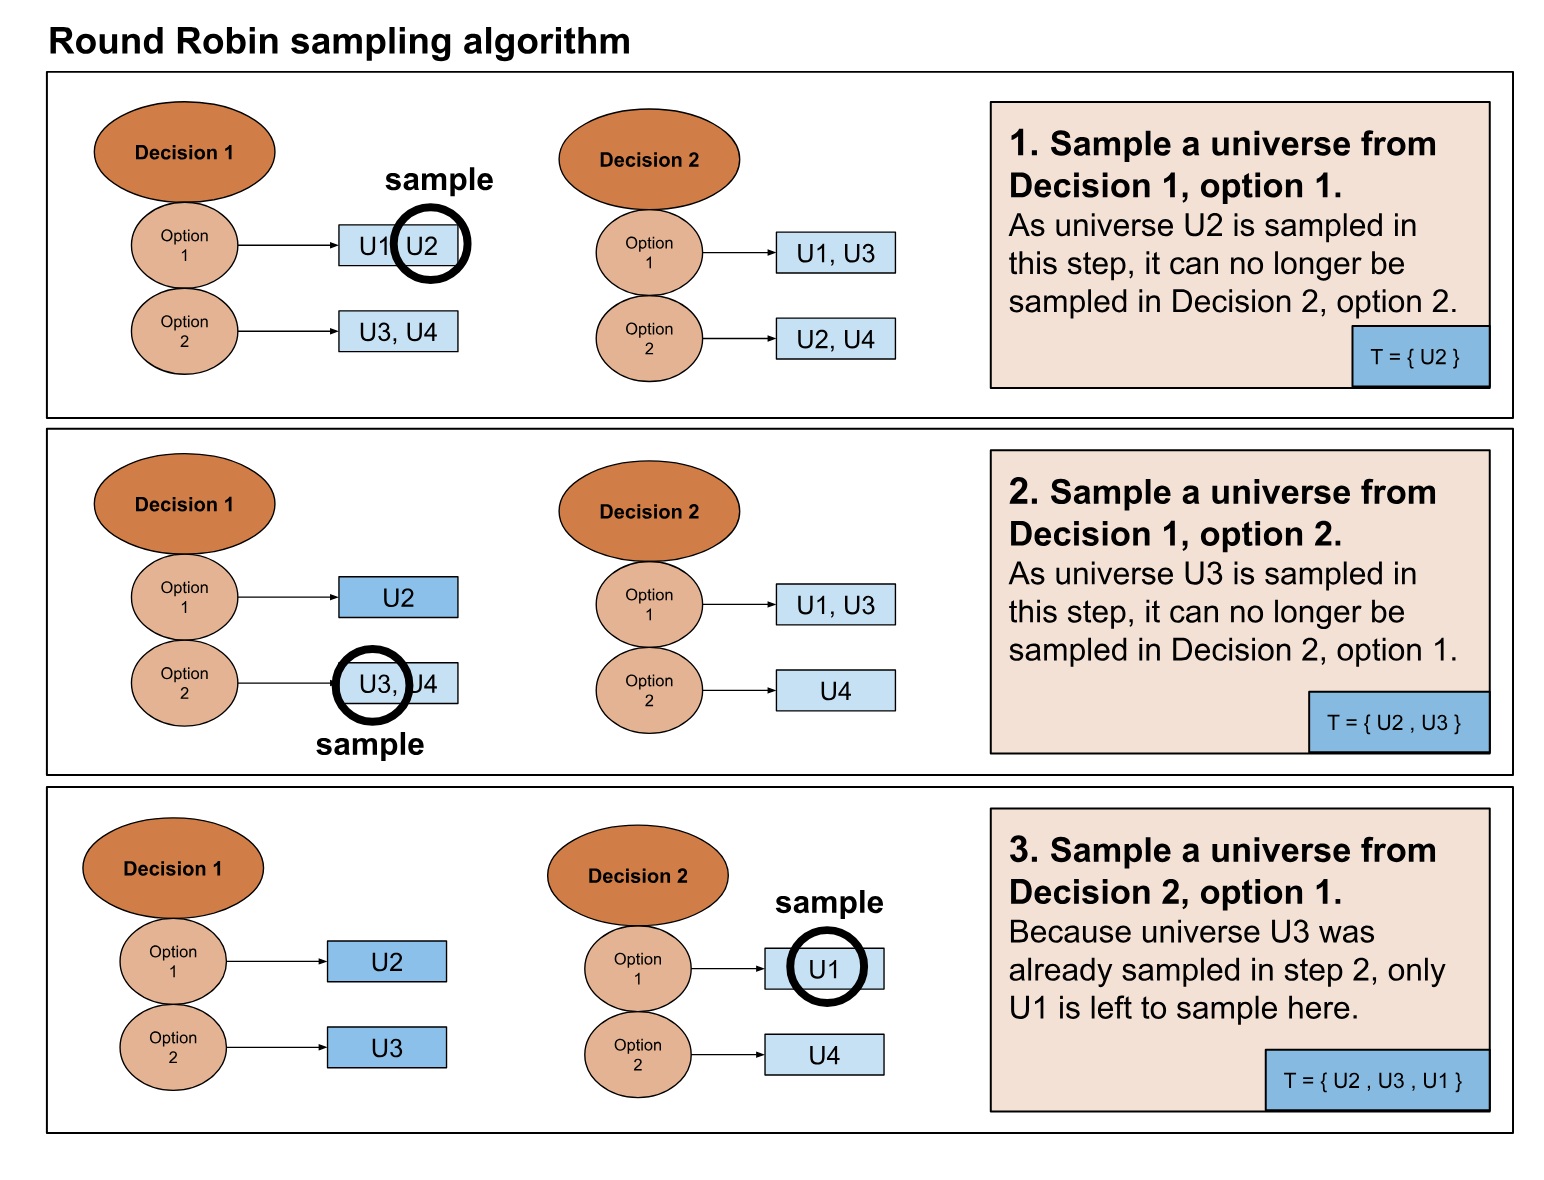
\includegraphics[width=1\linewidth,height=\textheight,keepaspectratio]{../figures/RoundRobinkleur.png}\hfill

\noindent \emph{Note.} \emph{U}~= universe, \emph{T} = the set of
sampled universes. Figure was created by L. Ubbink.

\end{figure}

Although Liu et al. (\citeproc{ref-liu_approximation_2023}{2023})
proposed sampling universes one by one and immediately processing the
multiverse results, in the present study, universes were selected
\emph{a priori} before running the multiverse analysis. The sampler was
implemented in two steps. First, decision options were mapped to
corresponding row numbers in the full decision space. Then, row numbers
were sampled according to the Round Robin algorithm and used to select
universes from the original decision space. This approach was more
computationally efficient than sampling directly from the decision
space. A random seed was set to ensure reproducibility.

To ensure sufficient data were available for each option to quantify
decision sensitivity, a minimum of 100 universes per option was sampled,
resulting in 6,400 sampled universes in total.

\subsection{Decision Sensitivity}\label{decision-sensitivity}

Two visual methods were used to explore the robustness of the multiverse
outcome distribution to different analytical specifications. First,
density plots were constructed to visualise the distribution of risk
ratios for each option within each analytical decision, as well as for
adjustment sets defined by the inclusion or exclusion of specific
confounders. Second, a specification curve was created by plotting each
universe against its estimated risk ratio, ordered from smallest to
largest (\citeproc{ref-simonsohn_specification_2015}{Simonsohn et al.,
2015}). Additionally, mean risk ratios were compared across options
within each decision to numerically explore observed patterns in more
detail.

Non-parametric k-sample Anderson-Darling tests were used to quantify the
decision sensitivity, as proposed by Liu et al.
(\citeproc{ref-liu_approximation_2023}{2023}). If RRs resulting from
\emph{k} options within a decision were found not to originate from the
same empirical cumulative distribution function, the decision was
classified as sensitive (\citeproc{ref-scholz_k-sample_1987}{Scholz \&
Stephens, 1987}). The AD statistic measures the weighted difference
between the ECDFs of \emph{k} samples, with emphasis on the tails of the
distributions, and is calculated as follows:

\begin{align}
  A_{kN}^2 = \frac{1}{N} \cdot \sum_{i=1}^k \frac{1}{n_i} \sum_{j=1}^{N-1} \frac{(N \cdot M_{ij} - j \cdot n_i)^2}{j(N - j)}
\end{align}

Where:

\begin{itemize}
\tightlist
\item
  \(N\) is the number of observations; the number of RRs resulting from
  all possible universes.
\item
  \(k\) is the number of groups; number of options per decision.
\item
  \(n_i\) is the number of observations per group; number or RRs
  resulting universes including a specific option.
\item
  \(Z_1 < ... < Z_N\) is the pooled ordered sample; all RRs ordered from
  lowest to highest.
\item
  \(j\) is the position in the pooled rank list \(Z_j\).
\item
  \(M_{ij}\) is the number of observations in a group that are smaller
  or equal to \(Z_j\).
\item
  \(j(N - j)\) is used to add heavier weigths to the tails of each
  distribution.
\end{itemize}

The standardised AD statistic (T.AD), which adjusts for number of groups
and sample size, was used for between-decision comparisons to evaluate
the relative sensitivity of each decision, where higher T.AD values
indicate more sensitive decisions. This statistic is calculated as
follows:

\begin{align}
  T_{kN} = \frac{A_{kN}^2 - (k - 1)}{\sigma_N}
\end{align}

For a more detailed calculation of \(\sigma_N\), the variance of
\(A_{kN}^2\), see Scholz and Stephens
(\citeproc{ref-scholz_k-sample_1987}{1987}, Equation 4).

Because there were sixty-four different adjustment sets, KS tests were
used for a more detailed evaluation of its decision sensitivity,
comparing risk ratio distributions for specifications including versus
excluding each adjustment variable. The KS test statistic (D) represents
the maximum absolute difference between the empirical cumulative
distribution functions of the two samples, ranging from 0 (identical) to
1 (no overlap). Values closer to 0 indicate a higher likelihood that the
two samples were drawn from the same distribution.

\subsection{Supplementary Materials}\label{supplementary-materials}

All analyses were conducted in R (version 4.4.2,
\citeproc{ref-r_core_team_r_2024}{Team, 2024}). All code scripts, with
sampler and multiverse functions, and package versions, can be found
\href{https://github.com/lodewijn/ManyAnalystThesisCompendium}{here}.

\section{Results}\label{results}

To evaluate the relative influence of each analytical decision on effect
size variability, a combination of descriptive and inferential methods
was used. First, some descriptive statistics of the underlying SHARE
data are reported, which were used to explore potential explanations for
the observed patterns. Then, general multiverse results are highlighted,
including model convergence rates and the overall distribution of effect
sizes across specifications, both visually and numerically. Finally, the
results of the decision sensitivity analyses are presented.

\subsection{Descriptive Statistics SHARE Data
Set}\label{descriptive-statistics-share-data-set}

Descriptive statistics about the SHARE data that was used for all
analyses can be found in Table~\ref{tbl-DescSHARE}. The number of people
who were married was about twice as high as the number of unmarried
people. It stood out that not all confounders were equally distributed
across groups. Married individuals were on average 4 years younger than
unmarried individuals (65 versus 69 years old). Additionally, the
distribution of sex differed between groups: 50.8\% of married
individuals were female, compared to 68.5\% in the unmarried group.

\begin{table}

{\caption{{Descriptive statistics of binary and numerical outcomes in
the SHARE data set.}{\label{tbl-DescSHARE}}}
\vspace{-20pt}}

\begingroup\fontsize{11}{13}\selectfont

\begin{longtable*}[t]{>{\raggedright\arraybackslash}p{5cm}>{\centering\arraybackslash}p{5cm}>{\centering\arraybackslash}p{5cm}}
\toprule
 & Unmarried & Married\\
\midrule
Number of people in group & 106,954 & 229,850\\
Mean age (years) & 69 & 65\\
Female (\%) & 68.5 & 50.8\\
Ever smoked (\%) & 44.8 & 46.6\\
Event ever (\%) & 17.1 & 14.1\\
Event since last interview (\%) & 4.9 & 3.9\\
Death by event (\%) & 23.6 & 24.3\\
Married before 18 (\%) & 0.0 & 1.5\\
Divorced or widowed (\%) & 26.9 & 0.0\\
From Israel (\%) & 2.9 & 3.7\\
Younger than 55 at W1 (\%) & 33.3 & 43.2\\
Born after 1954 (\%) & 18.4 & 24.0\\
\bottomrule
\end{longtable*}
\endgroup{}

\emph{Note.} Descriptives about categorical variables, such as level of
education, country and physical activity are not provided in this table.
For more information about these variables, see the original SHARE data.

\end{table}

\subsection{Model Convergence}\label{model-convergence}

Out of the 6,400 sampled universes, 1,487 failed to converge.
Non-convergence mostly occurred in log-binomial models (n = 1,102),
followed by generalised estimating equations (GEE; n = 221) and logistic
regression (n = 164). Non-convergence seemed to occur most often when
the adjustment sets increased in size. The other three model types (Cox,
mixed effects logistic, and discrete-time mixed effects) successfully
converged in all cases. Across other analytical decisions,
non-convergence was distributed approximately equally, suggesting these
decisions did not substantially affect model convergence. In total,
4,913 universes yielded valid risk ratio estimates. The number of
converged and non-converged universes per decision option can be found
in Table~\ref{tbl-RRfulltable}.

\begin{figure}

\caption{\label{fig-spec-curve}Specification curve where risk ratio
estimates are sorted in ascending order (upper panel). Blue estimates
are significant (p \textless{} .05); orange are non-significant. The
lower panel shows the analytical decisions underlying each
specification, with columns aligned to the estimates above.}

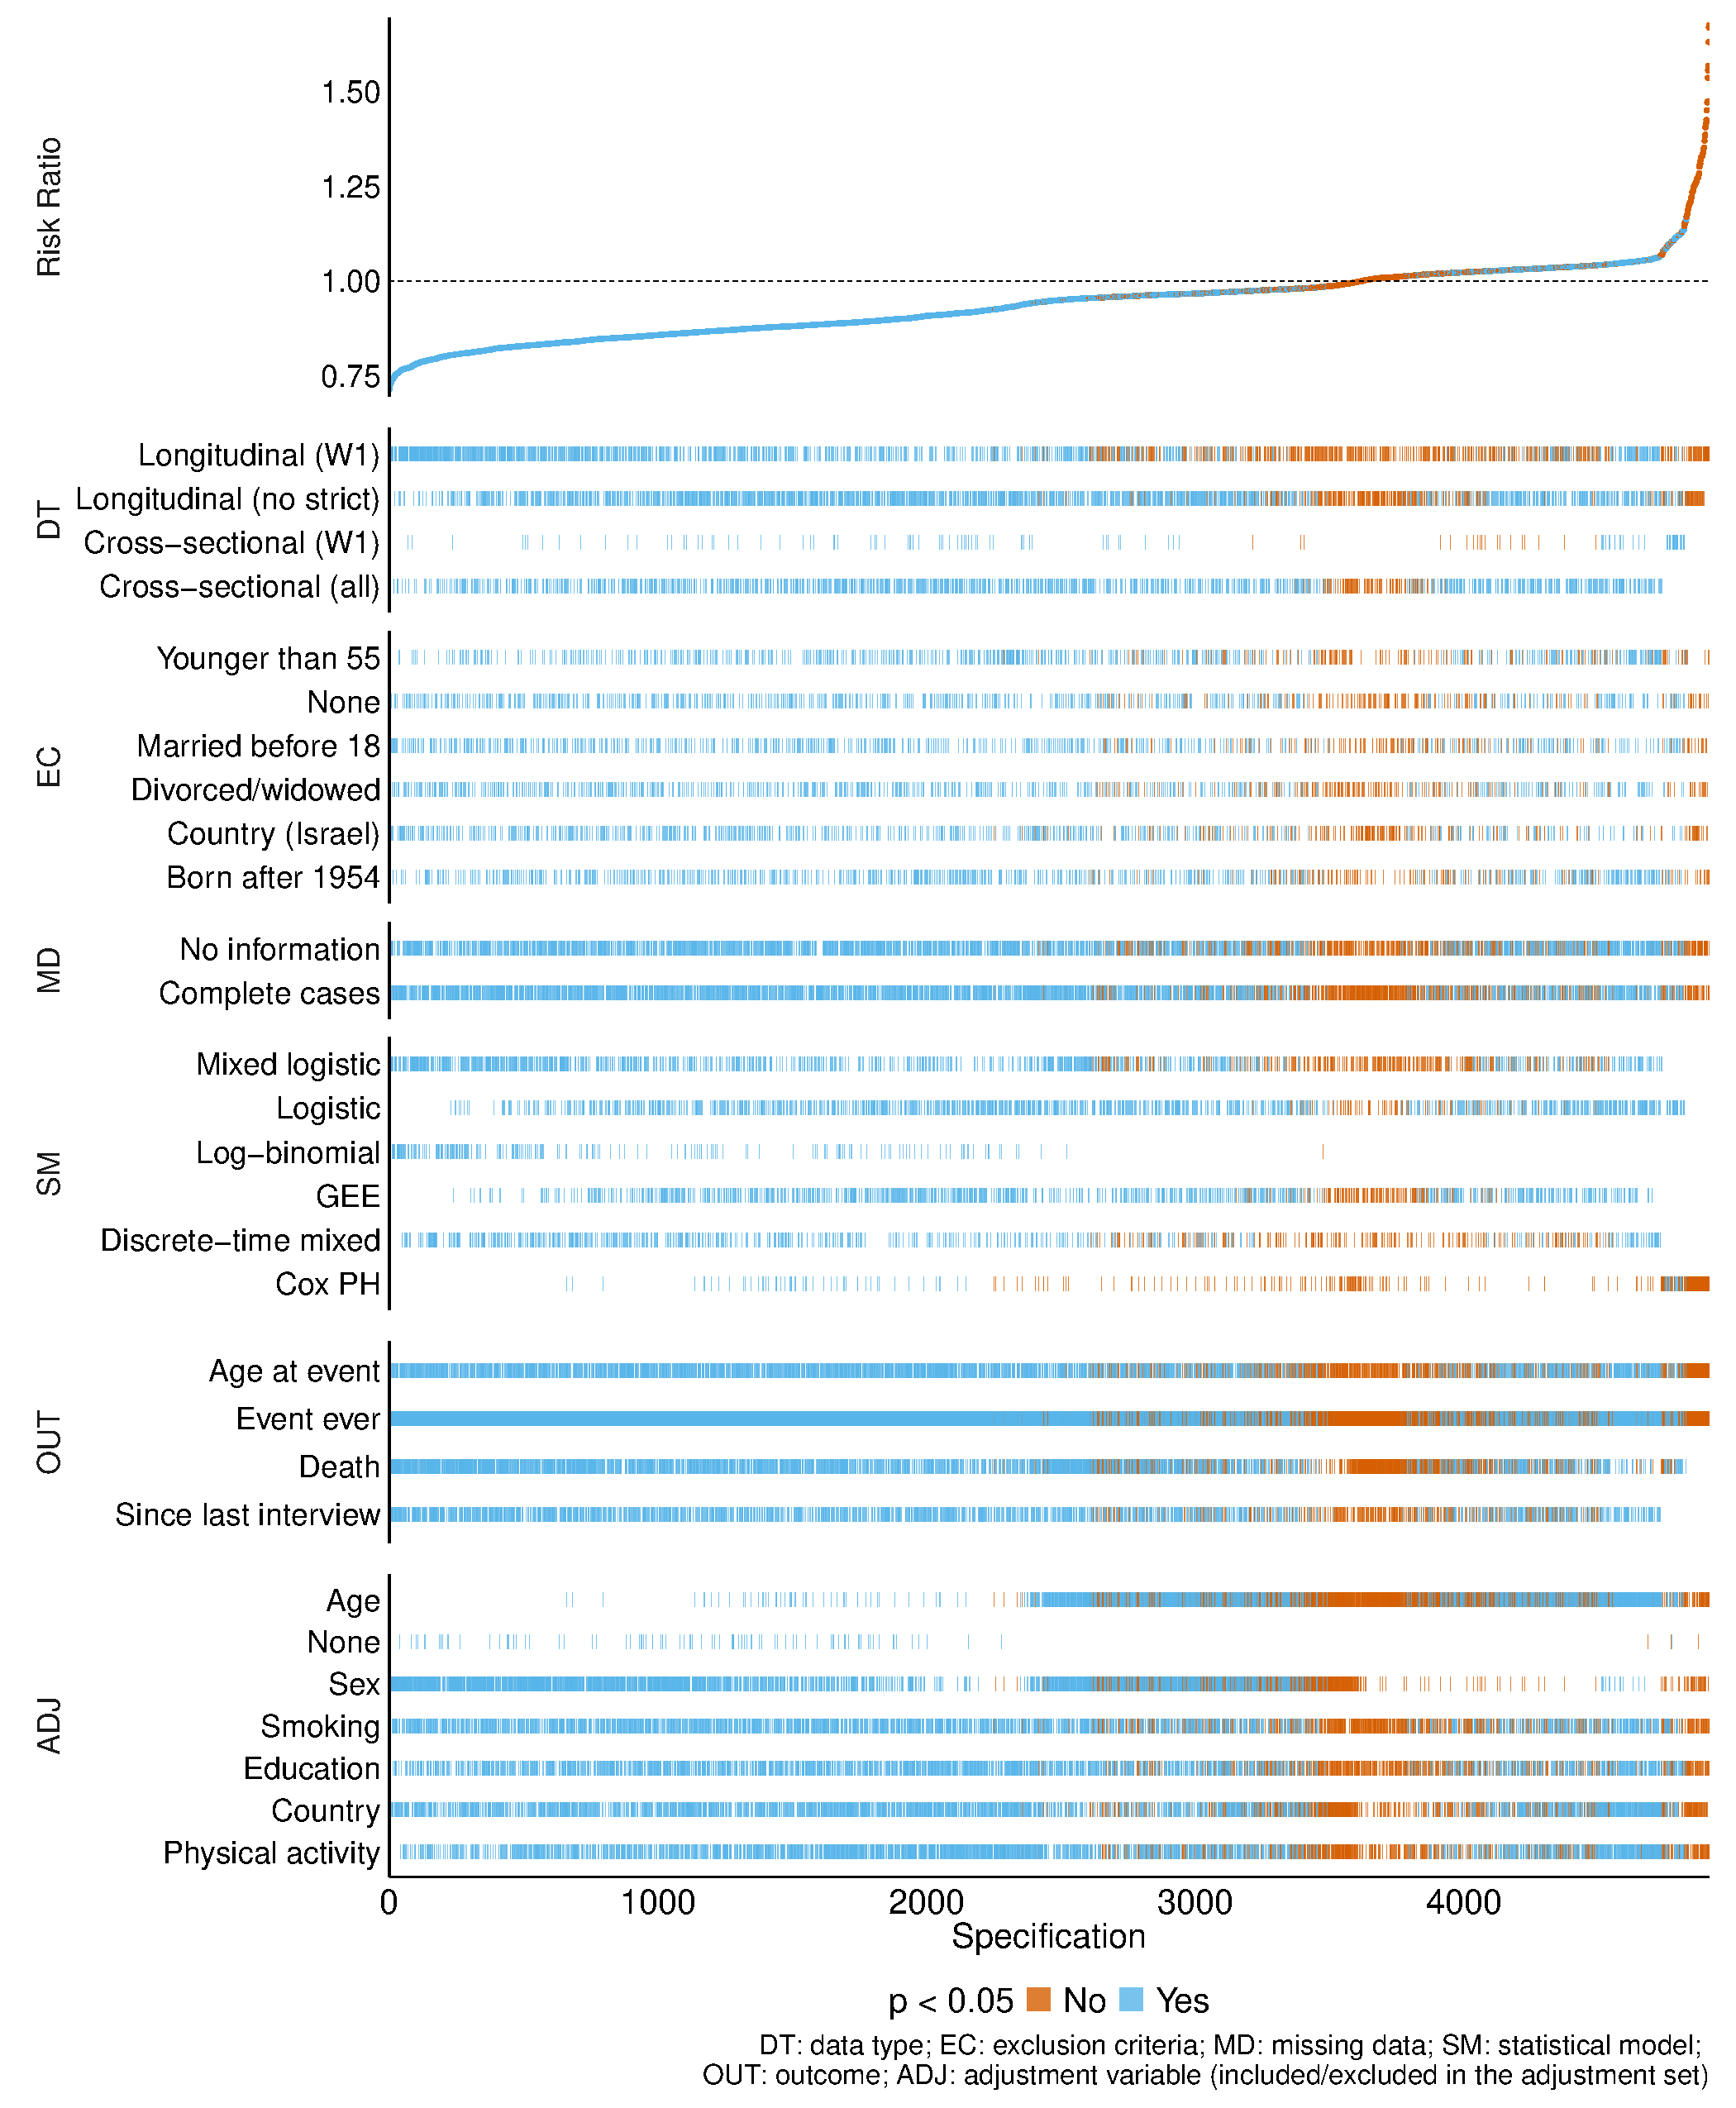
\includegraphics[width=1.5\linewidth,height=\textheight,keepaspectratio]{../figures/specification_curve.pdf}

\end{figure}%

\subsection{Overall Multiverse
Results}\label{overall-multiverse-results}

Across the 4,913 successful specifications, risk ratio estimates ranged
from 0.71 to 1.68 (median = 0.95, mean = 0.94, SD = 0.1), with 79.6\%
yielding significant results (p \textless{} .05). Of all converged
specifications, 65.3\% showed a statistically significant negative
association (RR \textless{} 1, p \textless{} .05), 14.3\% a
statistically significant positive association (RR \textgreater{} 1, p
\textless{} .05), and 20.4\% were non-significant. Within this sample of
the full multiverse, marriage thus appeared both as a protective factor
(RR \textless{} 1) and a risk factor (RR \textgreater{} 1) for
cardiovascular events, depending on the analytical specification.
Figure~\ref{fig-spec-curve} shows the full distribution of the effect
estimates across universes, arranged from smallest to largest risk
ratio, with significance indicated by colour.

Several patterns emerged in the specification curve
(Figure~\ref{fig-spec-curve}). First, universes including age as an
adjustment variable were clustered around higher RRs (mostly
\(\geq 1\)), while universes without age were clustered around lower RRs
(all \textless{} 1). When age was not controlled for, marriage thus
appeared a protective factor for cardiovascular events, while this
effect disappeared or even reversed when age was accounted for.

Second, the inclusion of sex as an adjustment variable showed roughly
the opposite pattern to age. Universes including sex were clustered
around lower RR values (almost all \(\leq\) 1), while those excluding
sex more often resulted in higher RRs. When sex was not accounted for,
the association was estimated across males and females simultaneously,
which appears to have attenuated the potential protective effect of
marriage.

Third, not including any covariates (ADJ-None in
Figure~\ref{fig-spec-curve}) always resulted in significantly negative
results (RR \textless{} 1). This means that the results of models not
adjusting for any covariates always suggested marriage had a protective
effect on cardiovascular outcomes.

Fourth, the highest RRs (\textgreater{} 1.25) only occurred in
specifications including Cox models, although almost none of these
estimates reached significance. Log-binomial models, in contrast,
yielded only RRs below 1, almost all of which were significant,
indicating a protective effect of marriage. Effect estimates seemed
robust to the other adjustment variables, all data types, missing data
handling, outcomes (except when combining outcome variables ``age at
event'' and ``event ever''), and exclusion criteria, with no clear
clustering patterns across these decisions.

\subsection{Decision Sensitivity}\label{decision-sensitivity-1}

Density plots were used to examine the effect size distributions across
decision options in more detail (see Figure~\ref{fig-dens-plot}). Data
type, missing data, exclusion criteria, and outcome showed largely
overlapping RR distributions across their options. However, in case of
statistical models and adjustment sets there were clear separations in
RR densities between options. Consistent with the patterns found in
Figure~\ref{fig-spec-curve}, log-binomial models were clustered below RR
values of 1, while the density of Cox showed a long tail extending above
1. Specifications that included age in the adjustment set showed a clear
shift towards higher RRs compared to those without age as a confounder.

\begin{figure}

\caption{\label{fig-dens-plot}Densities of risk ratios (RR) across
decisions and their options. All densities represent a different option
within a desicion. Panels are shown in greyscale when densities across
options largely overlap, indicating minimal variation between options.
Colours are only used in panels where differences between options were
visually substantial and therefore potentially influential for the
estimated RR.}

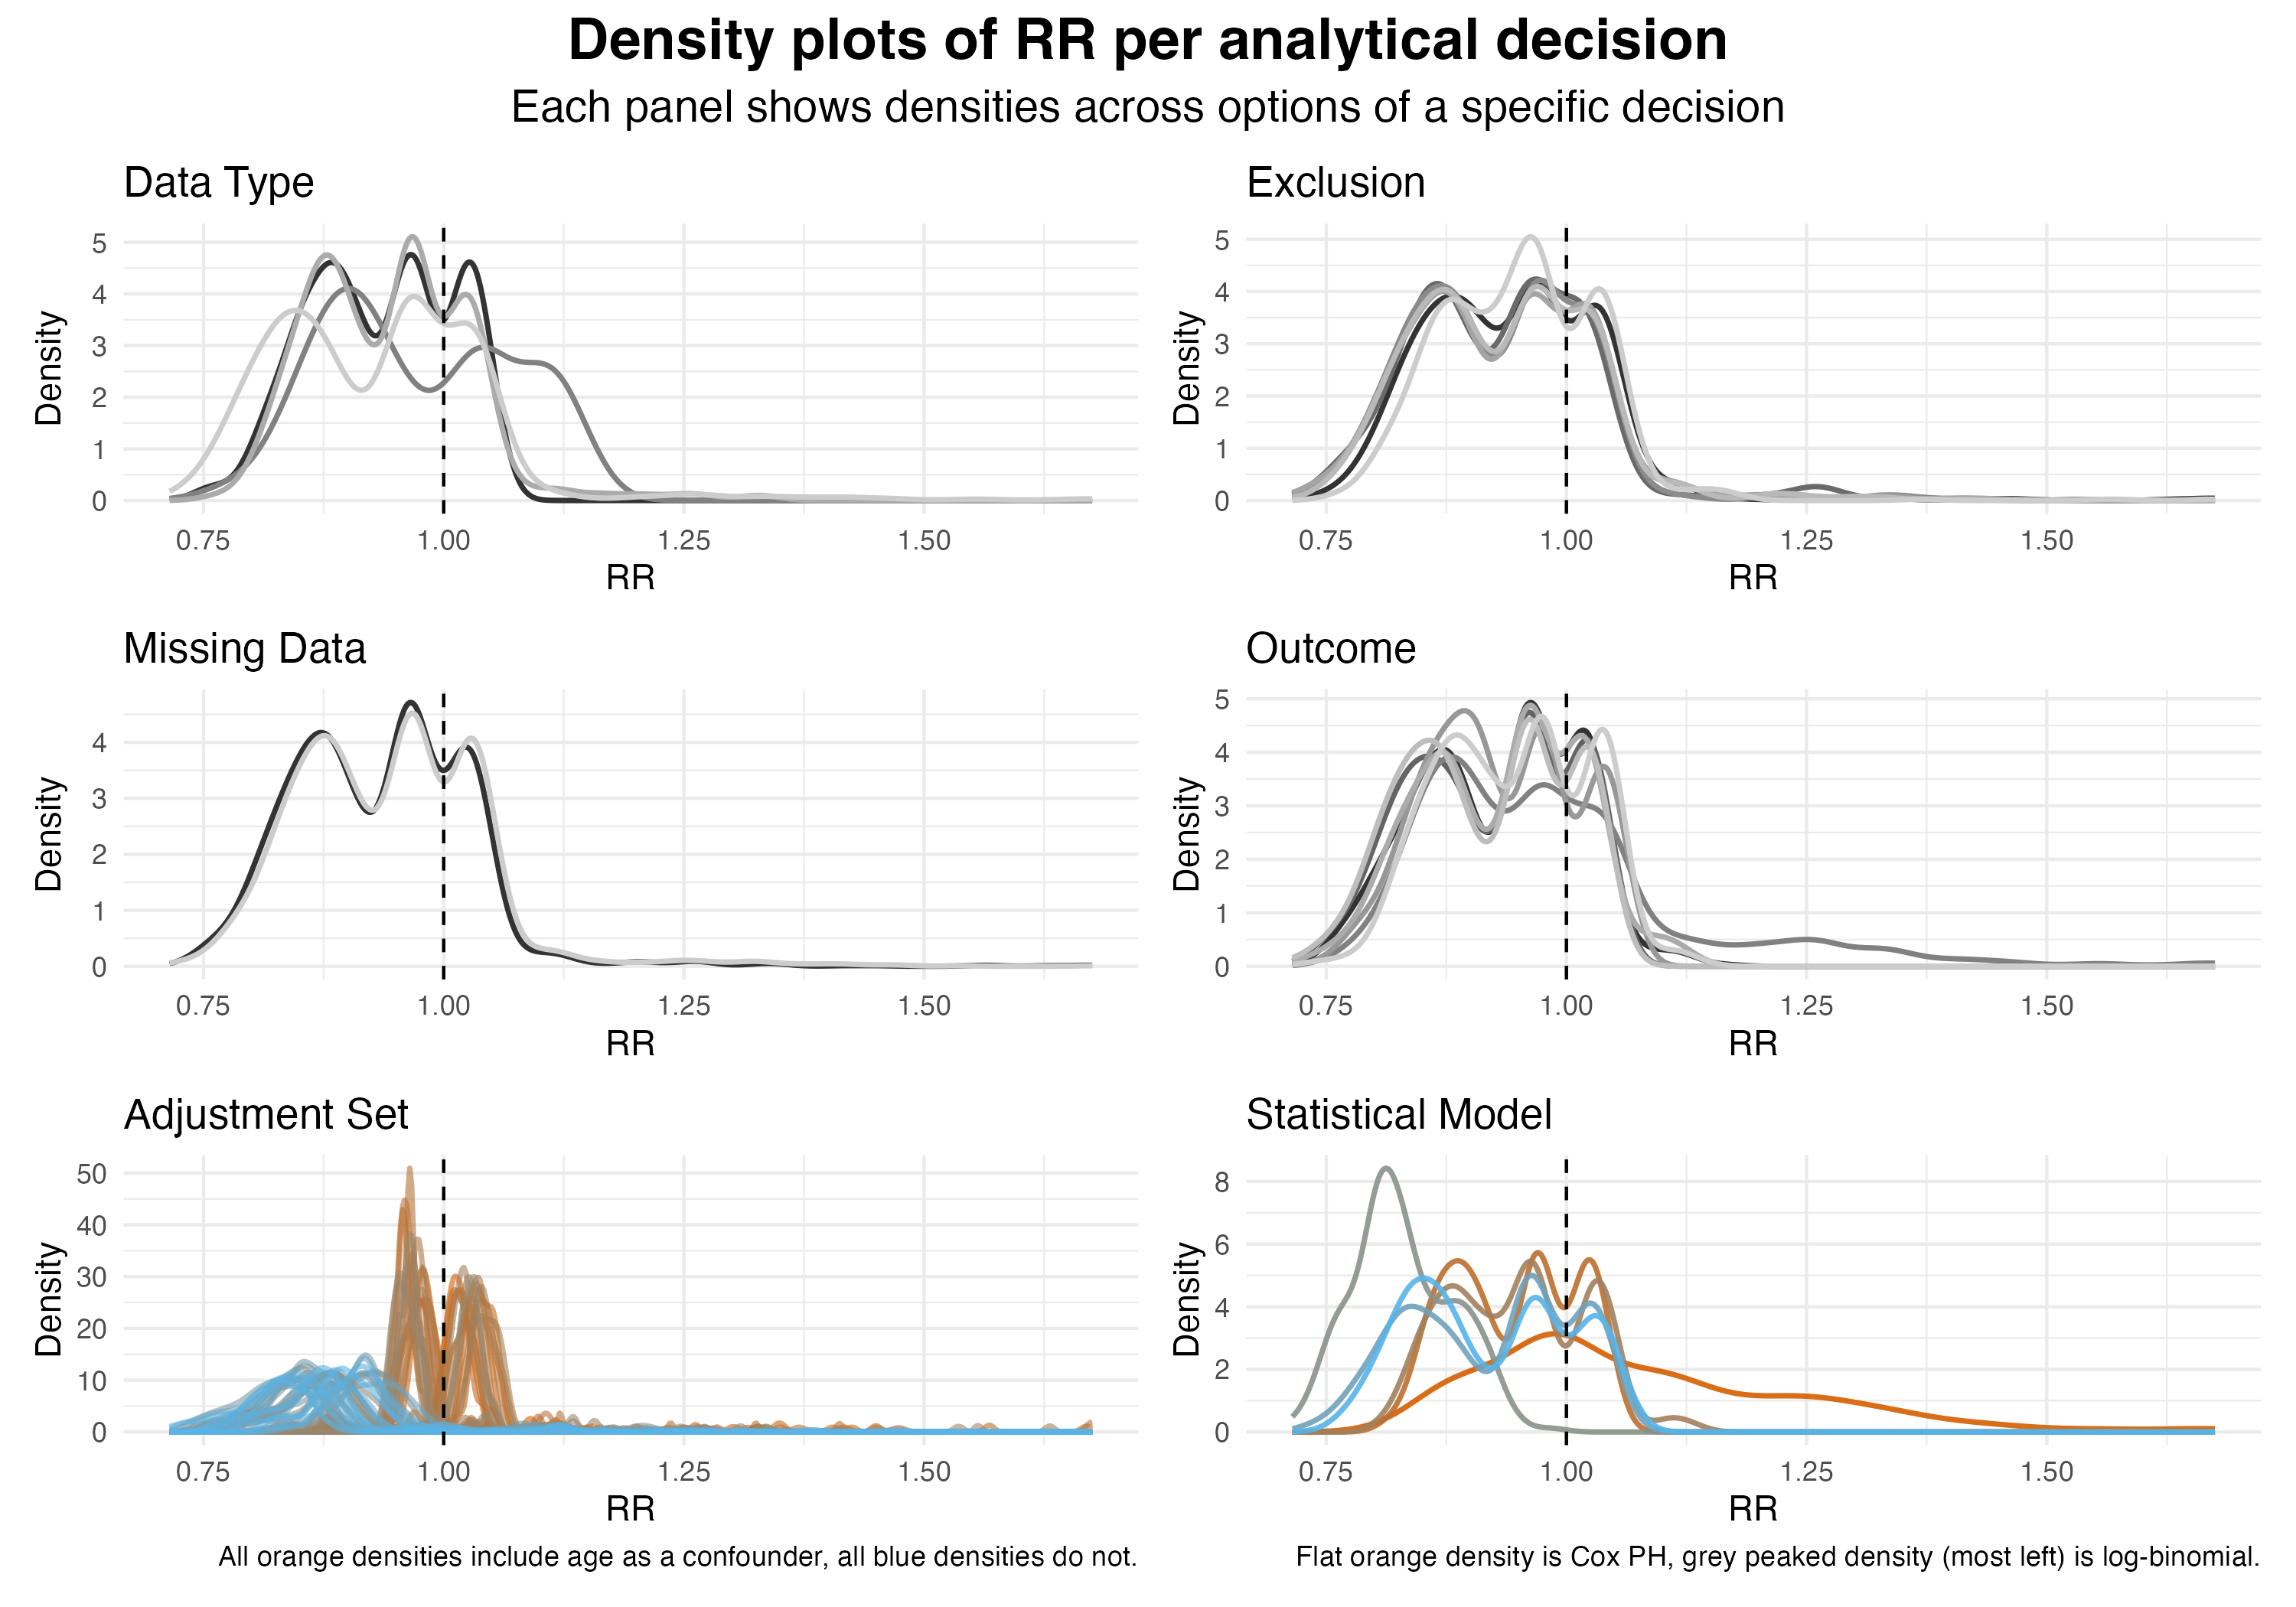
\includegraphics[width=1\linewidth,height=\textheight,keepaspectratio]{../figures/density_plot.png}

\end{figure}%

\begin{table}

{\caption{{K-sample Anderson-Darling Tests Across Analytical Decision
Options}{\label{tbl-ADtest}}}
\vspace{-20pt}}

\begingroup\fontsize{11}{13}\selectfont

\begin{longtable*}[t]{>{\raggedright\arraybackslash}p{5cm}>{\centering\arraybackslash}p{3cm}>{\centering\arraybackslash}p{3cm}>{\centering\arraybackslash}p{3cm}}
\toprule
Decision & k & T.AD & p-value\\
\midrule
Missing Data & 2 & 5.89 & .002\\
Exclusion Criteria & 6 & 13.13 & < .001\\
Data Type & 4 & 50.88 & < .001\\
Outcome & 7 & 52.26 & < .001\\
Statistical Model & 6 & 307.10 & < .001\\
Adjustment Set & 64 & 394.79 & < .001\\
\bottomrule
\end{longtable*}
\endgroup{}

\emph{Note.} Higher standardised AD values indicate more sensitive
decisions. \emph{k} = number of options; \emph{T.AD} = standardised AD
value.

\end{table}

Mean RR ranges across options confirmed the patterns found in the
specification curve and density plots (Table~\ref{tbl-RRfulltable} in
the Appendix). Statistical model (0.83--1.08) and adjustment set
(0.83--1.05) showed the largest variation in mean RR across options,
while other decisions showed smaller ranges: exclusion criteria
(0.94--0.94), missing data (0.93--0.95), data type (0.93--0.97), and
outcome (0.92--0.98).

A k-sample Anderson-Darling test (AD test) was used to quantify decision
sensitivity (for the ECDFs per decision see Figure~\ref{fig-ECDF} in the
Appendix). As shown in Table~\ref{tbl-ADtest}, AD tests for all
decisions were highly significant (almost all p \textless{} .001),
indicating distributional differences across options within each
decision. Adjustment set and statistical model showed substantially
higher T.AD values (307.1 and 394.79, respectively) than other decisions
(missing data: 5.89; exclusion: 13.13; outcome: 50.88; data type:
52.26). This indicates that statistical model and adjustment set had the
largest impact on the distribution of effect estimates. The number of
options per decision did not seem to substantially affect the T.AD
values.

Kolmogorov-Smirnov tests (KS test) were used to compare RR distributions
for specifications including versus excluding each adjustment variable.
For the ECDFs across adjustment variables, see
Figure~\ref{fig-ECDF-ADJ}. As can be seen in Table~\ref{tbl-KStest},
inclusion of all adjustment variables, except smoking, resulted in
significantly different distributions than when these variables were
excluded (p \textless{} .001). Age showed the largest effect (0.88),
followed by not including any confounders (0.54) and sex (0.45).
Physical activity, country, and education showed moderate, but
significant, effects (\(D_{activity}\) = 0.16, \(D_{country}\) = 0.1,
and \(D_{education}\) = 0.08). This confirms that the adjustment set
sensitivity seems to be driven primarily by age, sex and the decision
not to include confounders at all.

\begin{table}

{\caption{{Kolmogorov--Smirnov tests for distributional differences
across adjustment set options, and the number of universes each variable
was included or excluded in.}{\label{tbl-KStest}}}
\vspace{-20pt}}

\vspace{10pt}

\begingroup\fontsize{11}{13}\selectfont

\begin{tabular}[t]{>{\raggedright\arraybackslash}p{5cm}>{\centering\arraybackslash}p{2cm}>{\centering\arraybackslash}p{2cm}>{\centering\arraybackslash}p{2cm}>{\raggedleft\arraybackslash}p{2cm}}
\toprule
Adjustment variable & Included & Excluded & D & p-value\\
\midrule
Smoking & 2332 & 2581 & 0.03 & 0.341\\
Education & 2214 & 2699 & 0.08 & < .001\\
Country & 2436 & 2477 & 0.10 & < .001\\
Physical activity & 2431 & 2482 & 0.16 & < .001\\
Sex & 2409 & 2504 & 0.45 & < .001\\
None & 100 & 4813 & 0.54 & < .001\\
Age & 2330 & 2583 & 0.88 & < .001\\
\bottomrule
\end{tabular}
\endgroup{}

\vspace{6pt}

\emph{Note.} \emph{D} = KS test statistic (range 0 - 1), absolute max
distance between the ECDFs of the two samples, smaller numbers indicate
smaller distributional differences.

\end{table}

That adjustment set sensitivity is driven primarily by age, sex and not
including any confounders (when None was included), was also visible in
the RR density distributions (Figure~\ref{fig-dens-ADJ}). Including age
as an adjustment variable shifted the RR distribution to the right
(higher RRs), while including sex shifted it to the left (lower RRs).
The density pattern of specifications with no confounders resembled that
of specifications excluding age. This suggests that adjustment set
sensitivity was likely mainly driven by whether age was included at all,
which was consistent with the clustered pattern observed in the
specification curve (Figure~\ref{fig-spec-curve}). Other adjustment
variables did not result in pronounced differences between RR
distributions.

\begin{figure}

\caption{\label{fig-dens-ADJ}Densities of risk ratios (RR) across
inclusion/exclusion of different adjustment variables. Blue densities
indicate that the adjustment variable was included in the adjustment
set, orange densities indicate they were excluded. Including `None'
means no confounders were included in the analysis.}

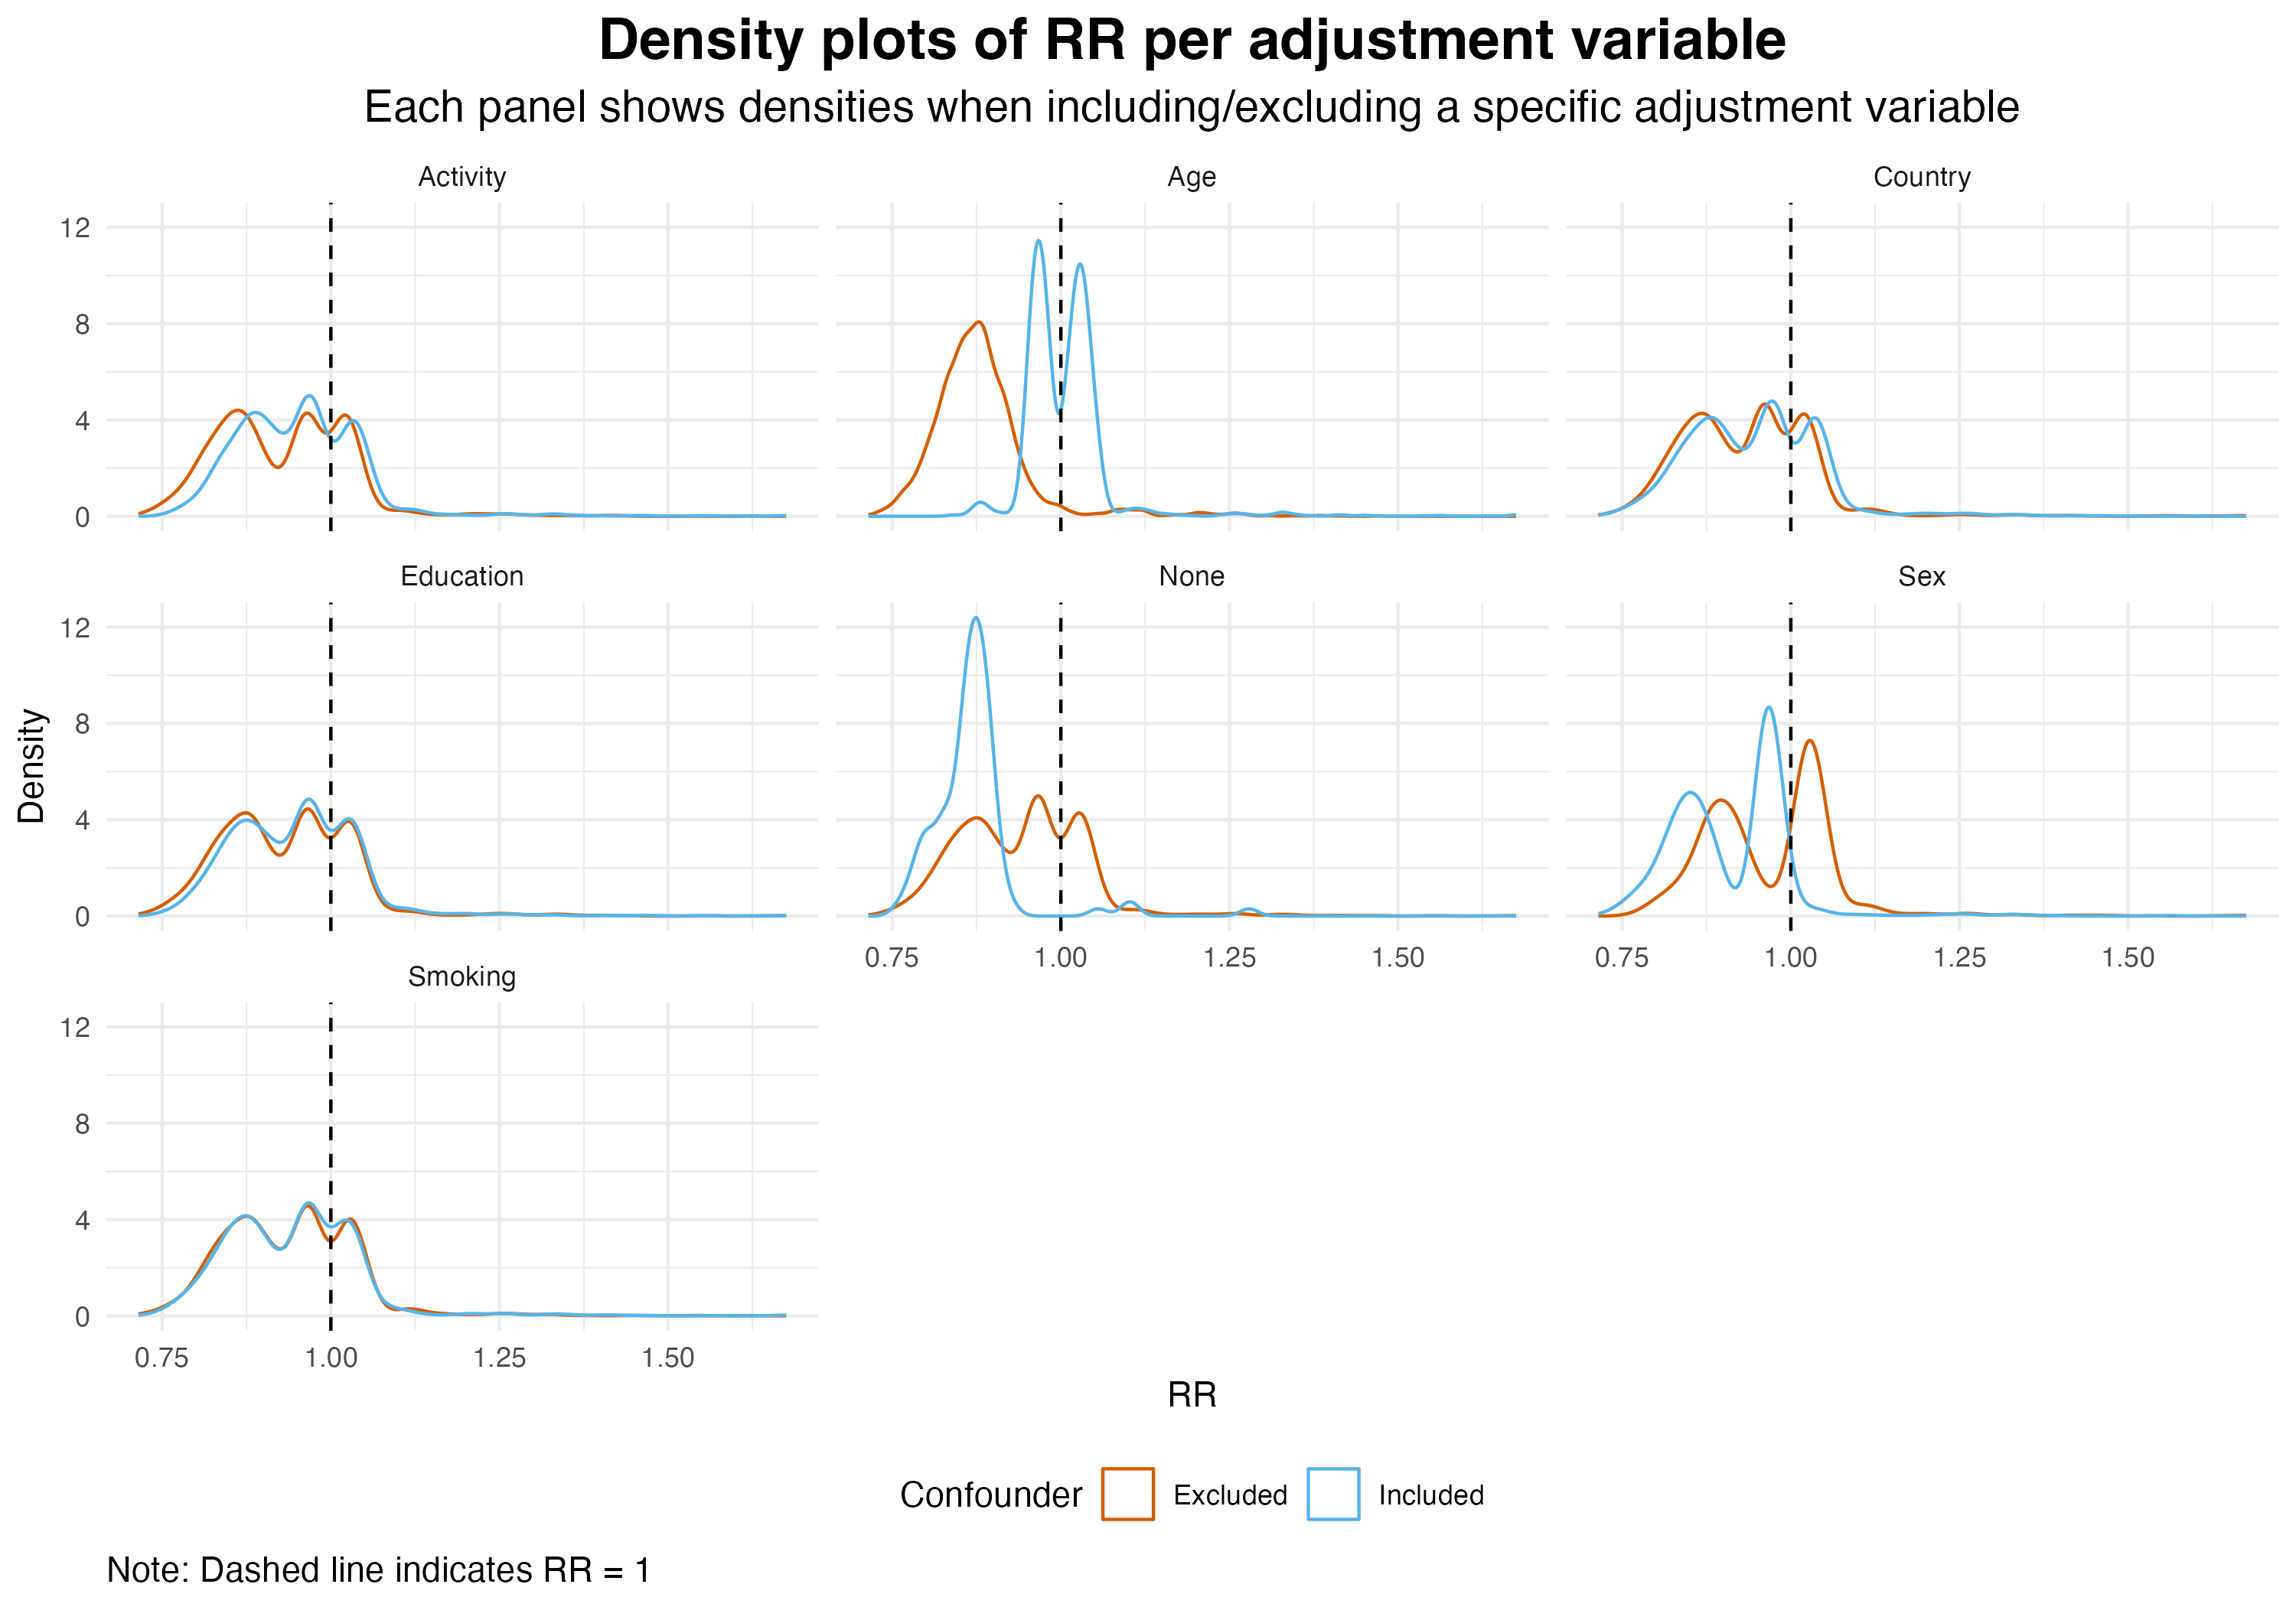
\includegraphics[width=1\linewidth,height=\textheight,keepaspectratio]{../figures/dens_per_confounder.png}

\end{figure}%

\section{Discussion}\label{discussion}

The present multiverse analysis aimed to quantify the relative
contribution of harmful versus helpful analytical decisions to effect
size variation for the association between marital status and
cardiovascular events, based on the many-analyst project by Kowall et
al. (\citeproc{ref-kowall_marital_2025}{2025}). Across 4,913
specifications, risk ratio estimates ranged from 0.71 to 1.68, with
79.6\% of the universes yielding significant results. Within the same
multiverse, marriage was found to be both significantly protective and
significantly harmful for cardiovascular health depending on the
analytical specification. This underscores that different analytical
pathways can lead to substantially different conclusions---a pattern
consistent with findings from earlier many-analyst projects
(\citeproc{ref-bastiaansen_time_2020}{Bastiaansen et al., 2020};
\citeproc{ref-botvinik-nezer_variability_2020}{Botvinik-Nezer et al.,
2020}; \citeproc{ref-breznau_observing_2022}{Breznau et al., 2022};
\citeproc{ref-gould_same_2025}{Gould et al., 2025};
\citeproc{ref-hoogeveen_many-analysts_2023}{Hoogeveen, Sarafoglou,
Aczel, et al., 2023}; \citeproc{ref-kowall_marital_2025}{Kowall et al.,
2025}; \citeproc{ref-silberzahn_many_2018}{Silberzahn et al., 2018}).

Although the Anderson-Darling tests showed statistically significant
distributional differences for all decisions, indicating they were all
sensitive, statistical model and adjustment set emerged as the most
prominent drivers of variation in RR distributions. All other decisions,
despite reaching statistical significance, showed minimal visual
distributional differences across options, suggesting their impact on
effect size variability was small. This was reinforced by the
descriptive plots and T.AD values, which suggest that only statistical
model and adjustment set had meaningful impact. When applying the
AB-framework classification, both a harmful source---statistical
model---and a helpful source---adjustment set---contributed meaningfully
to effect size variability.

\subsection{A Closer Examination of Helpful Sources of
Variation}\label{a-closer-examination-of-helpful-sources-of-variation}

A closer examination of adjustment set sensitivity using
Kolmogorov-Smirnov tests showed that age, sex, and not including any
confounders were the most important drivers of distributional
differences in the results. Consistent with the T.AD values, the pattern
observed for the no-confounders condition (Figure~\ref{fig-dens-ADJ}
when None was included) closely resembled that of the age-exclusion
condition, suggesting that age was the most important variable affecting
the decision sensitivity of the adjustment set. When no confounders were
included, risk ratio estimates were lower, and when any confounder was
included, the estimates shifted towards higher values. Age and sex
showed opposing patterns: controlling for age attenuated the protective
effect of marriage, while controlling for sex strengthened it.

A possible explanation for this pattern lies in the distribution of
these variables over the groups in the underlying data (see
Table~\ref{tbl-DescSHARE}). Unmarried individuals were on average four
years older (69 versus 65) and predominantly female (68.5\% versus
50.8\%), meaning the married and unmarried group differed systematically
in age and sex. The younger average age of married individuals may have
inflated the apparent protective effect of marriage, while the
relatively higher proportion of males in this group may have attenuated
it, given that men have greater cardiovascular risk
(\citeproc{ref-pana_sex-specific_2024}{Pana et al., 2024}). From a
causal inference perspective, the inclusion of covariates shifts the
estimation from a total effect to a direct effect
(\citeproc{ref-rohrer_thinking_2018}{Rohrer, 2018}). Adjusting for age,
for example, estimates the effect of marriage among people of the same
age. Without adjustment, the estimated effect of marriage on
cardiovascular events reflects not only the direct effect of marriage
itself, but also compositional differences between groups. This is a
good example of how selecting different covariates can result in
different questions being answered
(\citeproc{ref-simonsohn_specification_2015}{Simonsohn et al., 2015}).
The observed sensitivity to age and sex therefore reflects a genuine
difference in what is being estimated, and not arbitrary noise---the
kind of variation the AB-framework would characterise as helpful
(\citeproc{ref-auspurg_toward_2024}{Auspurg \& Brüderl, 2024}).

In contrast to the adjustment set, none of the other helpful sources of
variation meaningfully contributed to effect size differences. Outcome
variable choice had little influence on the distribution, with the
exception of ``age at event'' and ``event ever'' combined with Cox
models. However, this pattern more likely reflects the sensitivity of
the statistical model than the outcome operationalisation, given that
these outcomes were the only ones compatible with Cox and the higher
estimates did not occur with other models (see
Figure~\ref{fig-spec-curve}). The insensitivity to outcome choice may be
explained by the fact that all outcomes measure the same underlying
construct and are therefore expected to be highly correlated and
interchangeable, such that different operationalisations should yield
comparable effect sizes---which is consistent with the pattern observed
here (\citeproc{ref-avila_critical_2015}{Avila et al., 2015}). Some
exclusion criteria removed only a small proportion of participants
(\textless{} 4\%), and they were all distributed roughly equally across
groups (Table~\ref{tbl-DescSHARE}). Although this shows that the data
underlying both groups was likely comparable, it does not explain why
this decision showed little influence on the results. Additionally, it
was not clear why data type did not seem to heavily affect the results.
Future work should examine these findings more closely.

\newpage

\subsection{A Closer Examination of Harmful Sources of
Variation}\label{a-closer-examination-of-harmful-sources-of-variation}

When looking at harmful decisions, statistical models were the most
important drivers of effect size variation, with Cox and log-binomial
models resulting in visually different risk ratio distributions (see
Figure~\ref{fig-dens-plot}). Even after conversion to risk ratios, Cox
models consistently yielded substantially higher risk ratio estimates
than other modelling approaches, although these were often
non-significant, reflecting greater uncertainty in the estimates.
Log-binomial models, on the other hand, consistently resulted in low
risk ratios. Notably, model choice was not an independent decision in
this multiverse. For example, only three out of seven outcome
operationalisations contained time-to-event data, and only two out of
four data types were compatible with Cox models. Choosing this
statistical model therefore implicitly constrained other facets of the
analysis.

Log-binomial models also illustrate this inter-decision dependence
through their convergence behaviour. Of the fitted models, 1,102 failed
to converge, whereas only 232 were successful. Non-convergence occurred
most often when the adjustment sets increased in size, which connects to
a known limitation of the model (\citeproc{ref-zhu_refinements_2024}{Zhu
et al., 2024}). Log-binomial models restrict predicted disease
probabilities to lie between zero and one, which in turn bounds the
values the regression coefficients can take
(\citeproc{ref-williamson_log-binomial_2013}{Williamson et al., 2013}).
Convergence failure arises when the maximum likelihood solution sits on
the boundary of the parameter space, when at least one combination of
covariates results in an estimated probability of exactly one
(\citeproc{ref-zhu_refinements_2024}{Zhu et al., 2024}). This may become
more likely as adjustment sets grow, since larger sets may be more
likely to produce covariate combinations that hit this boundary.
Moreover, convergence behaviour for log-binomial models may be
software-specific
(\citeproc{ref-williamson_log-binomial_2013}{Williamson et al., 2013}).
In the present study, all analyses were conducted in R, meaning that
some of the observed non-convergence may even reflect software choices
rather than properties of the model itself. Choosing a log-binomial
model is therefore not an independent analytical decision, as its
convergence depends at least partly on size of the adjustment set and
the software that is used.

Another dependency arises with GEE models, which cannot handle missing
data and therefore force an explicit decision about missingness, whereas
other models default to complete-case analysis when nothing is
specified. Here, model selection again requires choices elsewhere in the
analytical pathway. Importantly, choices regarding missing data in
itself can also have implications that go beyond arbitrary noise. If
data are not missing at random, listwise deletion could result in not
including a subpopulation with a certain characteristic in the analysis.
Moreover, when confounders are missing not at random, causal effects are
not identifiable (\citeproc{ref-yang_causal_2019}{Yang et al., 2019}).

Taken together, these examples reveal a fundamental limitation of the
AB-framework: analytical decisions do not exist in isolation, so
categorising them as such is problematic. Decisions about statistical
models are entangled with data structure requirements, missing data
handling and variable operationalisation. This means that many harmful
decisions may in fact carry substantive assumptions that cannot be
separated from potential arbitrary variation the framework was designed
to identify.

\subsection{Comparison With Original Many-Analyst
Study}\label{comparison-with-original-many-analyst-study}

The range of effect sizes found in this study was broadly in line with
that of the original many-analyst project by Kowall et al.
(\citeproc{ref-kowall_marital_2025}{2025}), where effect sizes ranged
from 0.72 (OR) to 1.31 (HR). After applying the risk ratio conversions
used in the present study, the original effect sizes would correspond to
a range of approximately 0.85 to 1.21, indicating the original study
captured a slightly narrower range than the present multiverse. This is
not surprising, as the original study only included sixteen analyses,
compared to 4,913.

Despite the overlap in effect size ranges, the two studies diverged in
identifying impactful sources of variability. In contrast to the current
study, Kowall et al. (\citeproc{ref-kowall_marital_2025}{2025})
identified the data type (cross-sectional versus longitudinal) as the
main source of variation, with statistical model and adjustment set
playing only a minor role---the opposite of the present findings. This
inconsistency could reflect a fundamental difference between the two
approaches. Whereas Kowall et al.
(\citeproc{ref-kowall_marital_2025}{2025}) varied one decision at a
time, this multiverse analysis combined all decisions simultaneously and
evaluated their combined influence across the entire decision space.

Another potential explanation for the discrepancy between studies is the
finding that adjustment set sensitivity was driven primarily by age and
sex. In Kowall et al. (\citeproc{ref-kowall_marital_2025}{2025}), twelve
out of sixteen researchers included both age and sex in their analyses,
and the additional sensitivity analyses also held these variables
constant. Most researchers in the original study thus estimated the
direct effect of marriage on cardiovascular events, leaving little data
available about the effect of not including these confounders. This may
potentially have attenuated the observed sensitivity to adjustment set
decisions.

Rather than contradicting the original study, the present findings
extend it. When analytical decisions are varied jointly, instead of in
isolation, this can provide a different assessment of decision
sensitivity.

\subsection{Limitations and Future
Recommendations}\label{limitations-and-future-recommendations}

A first limitation concerns the inferential method used to assess
decision sensitivity. With 4,913 specifications, even minimal
distributional differences were statistically significant in the
k-sample Anderson-Darling test---implying it might be sensitive to
sample size. Consistent with Liu et al.
(\citeproc{ref-liu_approximation_2023}{2023}), AD tests effectively
yielded useful measures of between-decision sensitivity. However,
combining it with descriptive methods rather than relying on p-values
alone would provide a more informative picture of decision sensitivity.
Future research should also explore inferential methods that are less
susceptible to the large sample sizes characteristic of multiverse
analyses, explicitly account for the dependency structure between
decisions and specifications, and extend these approaches to allow the
derivation of a single result across uncertain decisions
(\citeproc{ref-aczel_consensus-based_2021}{Aczel et al., 2021}).

A second limitation is the generalisability of the present multiverse
results. The relative contribution of harmful versus helpful analytical
decisions will likely vary across studies, given the wide variety of
topics and research questions across many-analyst projects
(\citeproc{ref-gould_same_2025}{Gould et al., 2025};
\citeproc{ref-hoogeveen_many-analysts_2023}{Hoogeveen, Sarafoglou,
Aczel, et al., 2023}; \citeproc{ref-kowall_marital_2025}{Kowall et al.,
2025}; \citeproc{ref-silberzahn_many_2018}{Silberzahn et al., 2018}). It
does not seem realistic to expect that the results of this study will
directly apply to other projects. The decisions that proved to be most
influential here---statistical model and adjustment set---are not
necessarily the main sources of variation in other contexts, or even in
the same context when decisions are varied one at a time rather than
jointly, as the comparison with Kowall et al.
(\citeproc{ref-kowall_marital_2025}{2025}) illustrates. Conducting
multiverse analyses across different many-analyst projects, preferably
with a wide range of research questions and data structures, might
reveal more general patterns in decision sensitivity---although assuming
that such patterns exist may already be too bold.

A third limitation concerns the conversion of effect sizes. While this
has benefits for comparability across statistical models, the converged
risk ratios are always an approximation. According to VanderWeele
(\citeproc{ref-vanderweele_optimal_2020}{2020}), the square root
transformation of the odds ratio gives a reasonably good approximation
and differs from the true risk ratio by at most 25\%, when the
prevalence lies within 20\%--80\%. For hazard ratios, the conversion
will place the value within 16\% of the true risk ratios when the
prevalence lies within 20\%--80\%, and within 45\% if the prevalence is
between 10\%--90\%, which is the case in the present study. This
highlights that converting effect sizes, while useful for inter-model
comparisons, may simultaneously have introduced arbitrary variance in
the results.

More broadly, the current findings raise the question of what analysts
should do when analytical choices can fundamentally alter their
conclusions. Multiverse analysis cannot determine which specification is
``correct'', and the present study showed substantial variability in
effect estimates even within multiple defensible analytical paths. It is
therefore recommended that multiverse analysis is used not only as a
robustness check, but also as a transparent representation of the space
of plausible conclusions
(\citeproc{ref-botvinik-nezer_variability_2020}{Botvinik-Nezer et al.,
2020}). Moreover, researchers should ground their decisions in theory
and causal reasoning rather than idiosyncratic choices. Notably, only
three of the sixteen teams in Kowall et al.
(\citeproc{ref-kowall_marital_2025}{2025}) used directed acyclic graphs
(DAGs), and even those differed considerably. Pre-registering analytical
decisions, constructing DAGs prior to analysis, and making causal
assumptions explicit could help reduce unknown researcher degrees of
freedom (\citeproc{ref-botvinik-nezer_variability_2020}{Botvinik-Nezer
et al., 2020}). Combined with open research practices, this would not
eliminate analytical variability, but would ensure that it can be
assessed in a transparent manner to meaningfully interpret variation in
the results and their substantive conclusions.

\section{Conclusion}\label{conclusion}

This study investigated whether effect size variation in many-analyst
projects is driven primarily by harmful or helpful analytical decisions,
when they are systematically evaluated within a multiverse. Based on the
AB-framework, the results suggest that the answer is both. Statistical
model (harmful) and adjustment (helpful) emerged as the main drivers of
effect size variability across the 4,913 specifications, with risk
ratios ranging from significantly below 1 to significantly above 1,
corresponding to opposing substantive conclusions about the effect of
marriage on cardiovascular events. The sensitivity to adjustment set,
driven by the inclusion or exclusion of age and sex, illustrated that
differences in effect sizes reflected meaningful differences in what was
being estimated rather than arbitrary noise, underscoring the importance
of thinking carefully about causal structure prior to any analysis.
However, the current study has also revealed a limitation of the
AB-framework. Analytical decisions are rarely independent, making it
difficult to categorise them as purely harmful or helpful and attribute
variability to any single decision. This is precisely what makes
multiverse analysis valuable: rather than isolating individual
decisions, it captures how analytical choices jointly affect variability
in the results, making that variation transparent and interpretable.
Combining multiverse analysis with pre-registration, causal reasoning,
and open reporting practices would further strengthen the transparency
and credibility of empirical research---especially given ongoing
developments in sampling methods that make large-scale multiverses
increasingly computationally feasible
(\citeproc{ref-liu_approximation_2023}{Liu et al., 2023}).

\section{AI Statement}\label{ai-statement}

During this thesis, generative AI (Claude Sonnet 4.6, Claude Opus 4.6,
Claude Opus 4.7) was used for text editing/improving grammar and
assistance/debugging during coding.

\newpage

\section{References}\label{references}

\phantomsection\label{refs}
\begin{CSLReferences}{1}{0}
\bibitem[\citeproctext]{ref-aczel_consensus-based_2021}
Aczel, B., Szaszi, B., Nilsonne, G., Van Den Akker, O. R., Albers, C.
J., Van Assen, M. A., Bastiaansen, J. A., Benjamin, D., Boehm, U.,
Botvinik-Nezer, R., Bringmann, L. F., Busch, N. A., Caruyer, E.,
Cataldo, A. M., Cowan, N., Delios, A., Van Dongen, N. N., Donkin, C.,
Van Doorn, J. B., \ldots{} Wagenmakers, E.-J. (2021). Consensus-based
guidance for conducting and reporting multi-analyst studies.
\emph{eLife}, \emph{10}, e72185.
\url{https://doi.org/10.7554/eLife.72185}

\bibitem[\citeproctext]{ref-auspurg_toward_2024}
Auspurg, K., \& Brüderl, J. (2024). Toward a more credible assessment of
the credibility of science by many-analyst studies. \emph{Proceedings of
the National Academy of Sciences}, \emph{121}(38), e2404035121.
\url{https://doi.org/10.1073/pnas.2404035121}

\bibitem[\citeproctext]{ref-avila_critical_2015}
Avila, M. L., Stinson, J., Kiss, A., Brandão, L. R., Uleryk, E., \&
Feldman, B. M. (2015). A critical review of scoring options for clinical
measurement tools. \emph{BMC Research Notes}, \emph{8}(1), 612.
\url{https://doi.org/10.1186/s13104-015-1561-6}

\bibitem[\citeproctext]{ref-banks_editorial_2016}
Banks, G. C., Rogelberg, S. G., Woznyj, H. M., Landis, R. S., \& Rupp,
D. E. (2016). Editorial: {Evidence} on {Questionable} {Research}
{Practices}: {The} {Good}, the {Bad}, and the {Ugly}. \emph{Journal of
Business and Psychology}, \emph{31}(3), 323--338.
\url{https://doi.org/10.1007/s10869-016-9456-7}

\bibitem[\citeproctext]{ref-bastiaansen_time_2020}
Bastiaansen, J. A., Kunkels, Y. K., Blaauw, F. J., Boker, S. M.,
Ceulemans, E., Chen, M., Chow, S.-M., De Jonge, P., Emerencia, A. C.,
Epskamp, S., Fisher, A. J., Hamaker, E. L., Kuppens, P., Lutz, W.,
Meyer, M. J., Moulder, R., Oravecz, Z., Riese, H., Rubel, J., \ldots{}
Bringmann, L. F. (2020). Time to get personal? {The} impact of
researchers choices on the selection of treatment targets using the
experience sampling methodology. \emph{Journal of Psychosomatic
Research}, \emph{137}, 110211.
\url{https://doi.org/10.1016/j.jpsychores.2020.110211}

\bibitem[\citeproctext]{ref-borsch-supan_data_2013}
Börsch-Supan, A., Brandt, M., Hunkler, C., Kneip, T., Korbmacher, J.,
Malter, F., Schaan, B., Stuck, S., \& Zuber, S. (2013). Data {Resource}
{Profile}: {The} {Survey} of {Health}, {Ageing} and {Retirement} in
{Europe} ({SHARE}). \emph{International Journal of Epidemiology},
\emph{42}(4), 992--1001. \url{https://doi.org/10.1093/ije/dyt088}

\bibitem[\citeproctext]{ref-botvinik-nezer_variability_2020}
Botvinik-Nezer, R., Holzmeister, F., Camerer, C. F., Dreber, A., Huber,
J., Johannesson, M., Kirchler, M., Iwanir, R., Mumford, J. A., Adcock,
R. A., Avesani, P., Baczkowski, B. M., Bajracharya, A., Bakst, L., Ball,
S., Barilari, M., Bault, N., Beaton, D., Beitner, J., \ldots{}
Schonberg, T. (2020). Variability in the analysis of a single
neuroimaging dataset by many teams. \emph{Nature}, \emph{582}(7810),
84--88. \url{https://doi.org/10.1038/s41586-020-2314-9}

\bibitem[\citeproctext]{ref-breznau_observing_2022}
Breznau, N., Rinke, E. M., Wuttke, A., Nguyen, H. H. V., Adem, M.,
Adriaans, J., Alvarez-Benjumea, A., Andersen, H. K., Auer, D., Azevedo,
F., Bahnsen, O., Balzer, D., Bauer, G., Bauer, P. C., Baumann, M.,
Baute, S., Benoit, V., Bernauer, J., Berning, C., \ldots{} Żółtak, T.
(2022). Observing many researchers using the same data and hypothesis
reveals a hidden universe of uncertainty. \emph{Proceedings of the
National Academy of Sciences}, \emph{119}(44), e2203150119.
\url{https://doi.org/10.1073/pnas.2203150119}

\bibitem[\citeproctext]{ref-bulbulia_workflow_2023}
Bulbulia, J. A. (2023). A workflow for causal inference in
cross-cultural psychology. \emph{Religion, Brain \& Behavior},
\emph{13}(3), 291--306.
\url{https://doi.org/10.1080/2153599X.2022.2070245}

\bibitem[\citeproctext]{ref-del_giudice_travelers_2021}
Del Giudice, M., \& Gangestad, S. W. (2021). A {Traveler}'s {Guide} to
the {Multiverse}: {Promises}, {Pitfalls}, and a {Framework} for the
{Evaluation} of {Analytic} {Decisions}. \emph{Advances in Methods and
Practices in Psychological Science}, \emph{4}(1), 2515245920954925.
\url{https://doi.org/10.1177/2515245920954925}

\bibitem[\citeproctext]{ref-forbes_supporting_2023}
Forbes, H. J., Travers, J. C., \& Johnson, J. V. (2023). Supporting the
replication of your research. In \emph{Research {Ethics} in {Behavior}
{Analysis}} (pp. 237--262). Academic Press.
\url{https://doi.org/10.1016/B978-0-323-90969-3.00003-7}

\bibitem[\citeproctext]{ref-gould_same_2025}
Gould, E., Fraser, H. S., Parker, T. H., Nakagawa, S., Griffith, S. C.,
Vesk, P. A., Fidler, F., Hamilton, D. G., Abbey-Lee, R. N., Abbott, J.
K., Aguirre, L. A., Alcaraz, C., Aloni, I., Altschul, D., Arekar, K.,
Atkins, J. W., Atkinson, J., Baker, C. M., Barrett, M., \ldots{}
Zitomer, R. A. (2025). Same data, different analysts: Variation in
effect sizes due to analytical decisions in ecology and evolutionary
biology. \emph{BMC Biology}, \emph{23}(1), 35.
\url{https://doi.org/10.1186/s12915-024-02101-x}

\bibitem[\citeproctext]{ref-hoogeveen_many-analysts_2023}
Hoogeveen, S., Sarafoglou, A., Aczel, B., Aditya, Y., Alayan, A. J.,
Allen, P. J., Altay, S., Alzahawi, S., Amir, Y., Anthony, F.-V., Kwame
Appiah, O., Atkinson, Q. D., Baimel, A., Balkaya-Ince, M., Balsamo, M.,
Banker, S., Bartoš, F., Becerra, M., Beffara, B., \ldots{} Wagenmakers,
E.-J. (2023). A many-analysts approach to the relation between
religiosity and well-being. \emph{Religion, Brain \& Behavior},
\emph{13}(3), 237--283.
\url{https://doi.org/10.1080/2153599X.2022.2070255}

\bibitem[\citeproctext]{ref-hoogeveen_many-analysts_2023-1}
Hoogeveen, S., Sarafoglou, A., Van Elk, M., \& Wagenmakers, E.-J.
(2023). Many-analysts religion project: Reflection and conclusion.
\emph{Religion, Brain \& Behavior}, \emph{13}(3), 356--363.
\url{https://doi.org/10.1080/2153599X.2022.2070263}

\bibitem[\citeproctext]{ref-huang_development_2022}
Huang, Q., Wang, Y., \& et., al. (2022a). Development and introduction
of online evidence-based medicine research helper. \emph{CHINESE JOURNAL
OF EVIDENCE-BASED MEDICINE}, \emph{22}(12), 1483--1488.
\url{https://ebm-helper.cn/en/Conv/OR_RR.html}

\bibitem[\citeproctext]{ref-huang_development_2022-1}
Huang, Q., Wang, Y., \& et., al. (2022b). Development and introduction
of online evidence-based medicine research helper. \emph{CHINESE JOURNAL
OF EVIDENCE-BASED MEDICINE}, \emph{22}(12), 1483--1488.
\url{https://ebm-helper.cn/en/Conv/HR_RR.html}

\bibitem[\citeproctext]{ref-kowall_marital_2025}
Kowall, B., Ahrenfeldt, L. J., Basten, J., Becher, H., Brand, T., Braun,
J., Casjens, S., Claessen, H., Denz, R., Diebner, H. H., Diexer, S.,
Eisemann, N., Furrer, E., Galetzka, W., Girschik, C., Karch, A.,
Mikolajczyk, R., Peters, M., Rospleszcz, S., \ldots{} Rübsamen, N.
(2025). Marital status and risk of cardiovascular disease -- a
multi-analyst study in epidemiology. \emph{European Journal of
Epidemiology}, \emph{40}(5), 497--509.
\url{https://doi.org/10.1007/s10654-025-01235-8}

\bibitem[\citeproctext]{ref-kummerfeld_one_2023}
Kummerfeld, E., \& Jones, G. L. (2023). One data set, many analysts:
{Implications} for practicing scientists. \emph{Frontiers in
Psychology}, \emph{14}, 1094150.
\url{https://doi.org/10.3389/fpsyg.2023.1094150}

\bibitem[\citeproctext]{ref-liu_approximation_2023}
Liu, Y., Althoff, T., \& Heer, J. (2023). \emph{Approximation and
{Progressive} {Display} of {Multiverse} {Analyses}}. arXiv.
\url{https://doi.org/10.48550/arXiv.2305.08323}

\bibitem[\citeproctext]{ref-pana_sex-specific_2024}
Pana, T. A., Mamas, M. A., Wareham, N. J., Khaw, K.-T., Dawson, D. K.,
\& Myint, P. K. (2024). Sex-specific lifetime risk of cardiovascular
events: The {European} {Prospective} {Investigation} into
{Cancer}-{Norfolk} prospective population cohort study. \emph{European
Journal of Preventive Cardiology}, \emph{31}(2), 230--241.
\url{https://doi.org/10.1093/eurjpc/zwad283}

\bibitem[\citeproctext]{ref-rohrer_thinking_2018}
Rohrer, J. M. (2018). Thinking {Clearly} {About} {Correlations} and
{Causation}: {Graphical} {Causal} {Models} for {Observational} {Data}.
\emph{Advances in Methods and Practices in Psychological Science},
\emph{1}(1), 27--42. \url{https://doi.org/10.1177/2515245917745629}

\bibitem[\citeproctext]{ref-rohrer_what_2025}
Rohrer, J. M., Smith, G. D., \& Munafò, M. (2025). What can be learned
when multiple analysts arrive at different estimates. \emph{European
Journal of Epidemiology}, \emph{40}(5), 493--495.
\url{https://doi.org/10.1007/s10654-025-01249-2}

\bibitem[\citeproctext]{ref-scholz_k-sample_1987}
Scholz, F. W., \& Stephens, M. A. (1987). \emph{K-{Sample}
{Anderson}-{Darling} {Tests}}.

\bibitem[\citeproctext]{ref-share-eric_survey_2024}
SHARE-ERIC. (2024a). \emph{Survey of {Health}, {Ageing} and {Retirement}
in {Europe} ({SHARE}) {Wave} 1}. SHARE-ERIC.
\url{https://doi.org/10.6103/SHARE.W1.900}

\bibitem[\citeproctext]{ref-share-eric_survey_2024-1}
SHARE-ERIC. (2024b). \emph{Survey of {Health}, {Ageing} and {Retirement}
in {Europe} ({SHARE}) {Wave} 2}. SHARE-ERIC.
\url{https://doi.org/10.6103/SHARE.W2.900}

\bibitem[\citeproctext]{ref-share-eric_survey_2024-2}
SHARE-ERIC. (2024c). \emph{Survey of {Health}, {Ageing} and {Retirement}
in {Europe} ({SHARE}) {Wave} 4}. SHARE-ERIC.
\url{https://doi.org/10.6103/SHARE.W4.900}

\bibitem[\citeproctext]{ref-share-eric_survey_2024-3}
SHARE-ERIC. (2024d). \emph{Survey of {Health}, {Ageing} and {Retirement}
in {Europe} ({SHARE}) {Wave} 5}. SHARE-ERIC.
\url{https://doi.org/10.6103/SHARE.W5.900}

\bibitem[\citeproctext]{ref-share-eric_survey_2024-4}
SHARE-ERIC. (2024e). \emph{Survey of {Health}, {Ageing} and {Retirement}
in {Europe} ({SHARE}) {Wave} 6}. SHARE-ERIC.
\url{https://doi.org/10.6103/SHARE.W6.900}

\bibitem[\citeproctext]{ref-share-eric_survey_2024-5}
SHARE-ERIC. (2024f). \emph{Survey of {Health}, {Ageing} and {Retirement}
in {Europe} ({SHARE}) {Wave} 7}. SHARE-ERIC.
\url{https://doi.org/10.6103/SHARE.W7.900}

\bibitem[\citeproctext]{ref-silberzahn_many_2018}
Silberzahn, R., Uhlmann, E. L., Martin, D. P., Anselmi, P., Aust, F.,
Awtrey, E., Bahník, Š., Bai, F., Bannard, C., Bonnier, E., Carlsson, R.,
Cheung, F., Christensen, G., Clay, R., Craig, M. A., Dalla Rosa, A.,
Dam, L., Evans, M. H., Flores Cervantes, I., \ldots{} Nosek, B. A.
(2018). Many {Analysts}, {One} {Data} {Set}: {Making} {Transparent}
{How} {Variations} in {Analytic} {Choices} {Affect} {Results}.
\emph{Advances in Methods and Practices in Psychological Science},
\emph{1}(3), 337--356. \url{https://doi.org/10.1177/2515245917747646}

\bibitem[\citeproctext]{ref-simonsohn_specification_2015}
Simonsohn, U., Simmons, J. P., \& Nelson, L. D. (2015). Specification
{Curve}: {Descriptive} and {Inferential} {Statistics} on {All}
{Reasonable} {Specifications}. \emph{SSRN Electronic Journal}.
\url{https://doi.org/10.2139/ssrn.2694998}

\bibitem[\citeproctext]{ref-steegen_increasing_2016}
Steegen, S., Tuerlinckx, F., Gelman, A., \& Vanpaemel, W. (2016).
Increasing {Transparency} {Through} a {Multiverse} {Analysis}.
\emph{Perspectives on Psychological Science}, \emph{11}(5), 702--712.
\url{https://doi.org/10.1177/1745691616658637}

\bibitem[\citeproctext]{ref-r_core_team_r_2024}
Team, R. C. (2024). \emph{R: {A} {Language} and {Environment} for
{Statistical} {Computing}}. R Foundation for Statistical Computing.
\url{https://www.R-project.org/}

\bibitem[\citeproctext]{ref-vanderweele_optimal_2020}
VanderWeele, T. J. (2020). Optimal approximate conversions of odds
ratios and hazard ratios to risk ratios. \emph{Biometrics},
\emph{76}(3), 746--752. \url{https://doi.org/10.1111/biom.13197}

\bibitem[\citeproctext]{ref-williamson_log-binomial_2013}
Williamson, T., Eliasziw, M., \& Fick, G. H. (2013). Log-binomial
models: Exploring failed convergence. \emph{Emerging Themes in
Epidemiology}, \emph{10}, 14.
\url{https://doi.org/10.1186/1742-7622-10-14}

\bibitem[\citeproctext]{ref-yang_causal_2019}
Yang, S., Wang, L., \& Ding, P. (2019). Causal inference with
confounders missing not at random. \emph{Biometrika}, \emph{106}(4),
875--888. \url{https://doi.org/10.1093/biomet/asz048}

\bibitem[\citeproctext]{ref-zhang_whats_1998}
Zhang, J., \& Yu, K. F. (1998). What's the relative risk? {A} method of
correcting the odds ratio in cohort studies of common outcomes.
\emph{JAMA}, \emph{280}(19), 1690--1691.
\url{https://doi.org/10.1001/jama.280.19.1690}

\bibitem[\citeproctext]{ref-zhu_refinements_2024}
Zhu, C., Hosmer, D. W., Stankovich, J., Wills, K., \& Blizzard, L.
(2024). Refinements on the exact method to solve the numerical
difficulties in fitting the log binomial regression model for estimating
relative risk. \emph{Communications in Statistics - Theory and Methods},
\emph{53}(23), 8359--8375.
\url{https://doi.org/10.1080/03610926.2023.2284674}

\end{CSLReferences}

\appendix

\section{Empirical Cumulative Distribution Functions Across
Decisions}\label{apx-empirical-cumulative-distribution-functions-across-decisions}

\begin{figure}[H]

\caption{\label{fig-ECDF}Empirical cumulative distribution functions of
risk ratios (RR) across decisions and their options.}

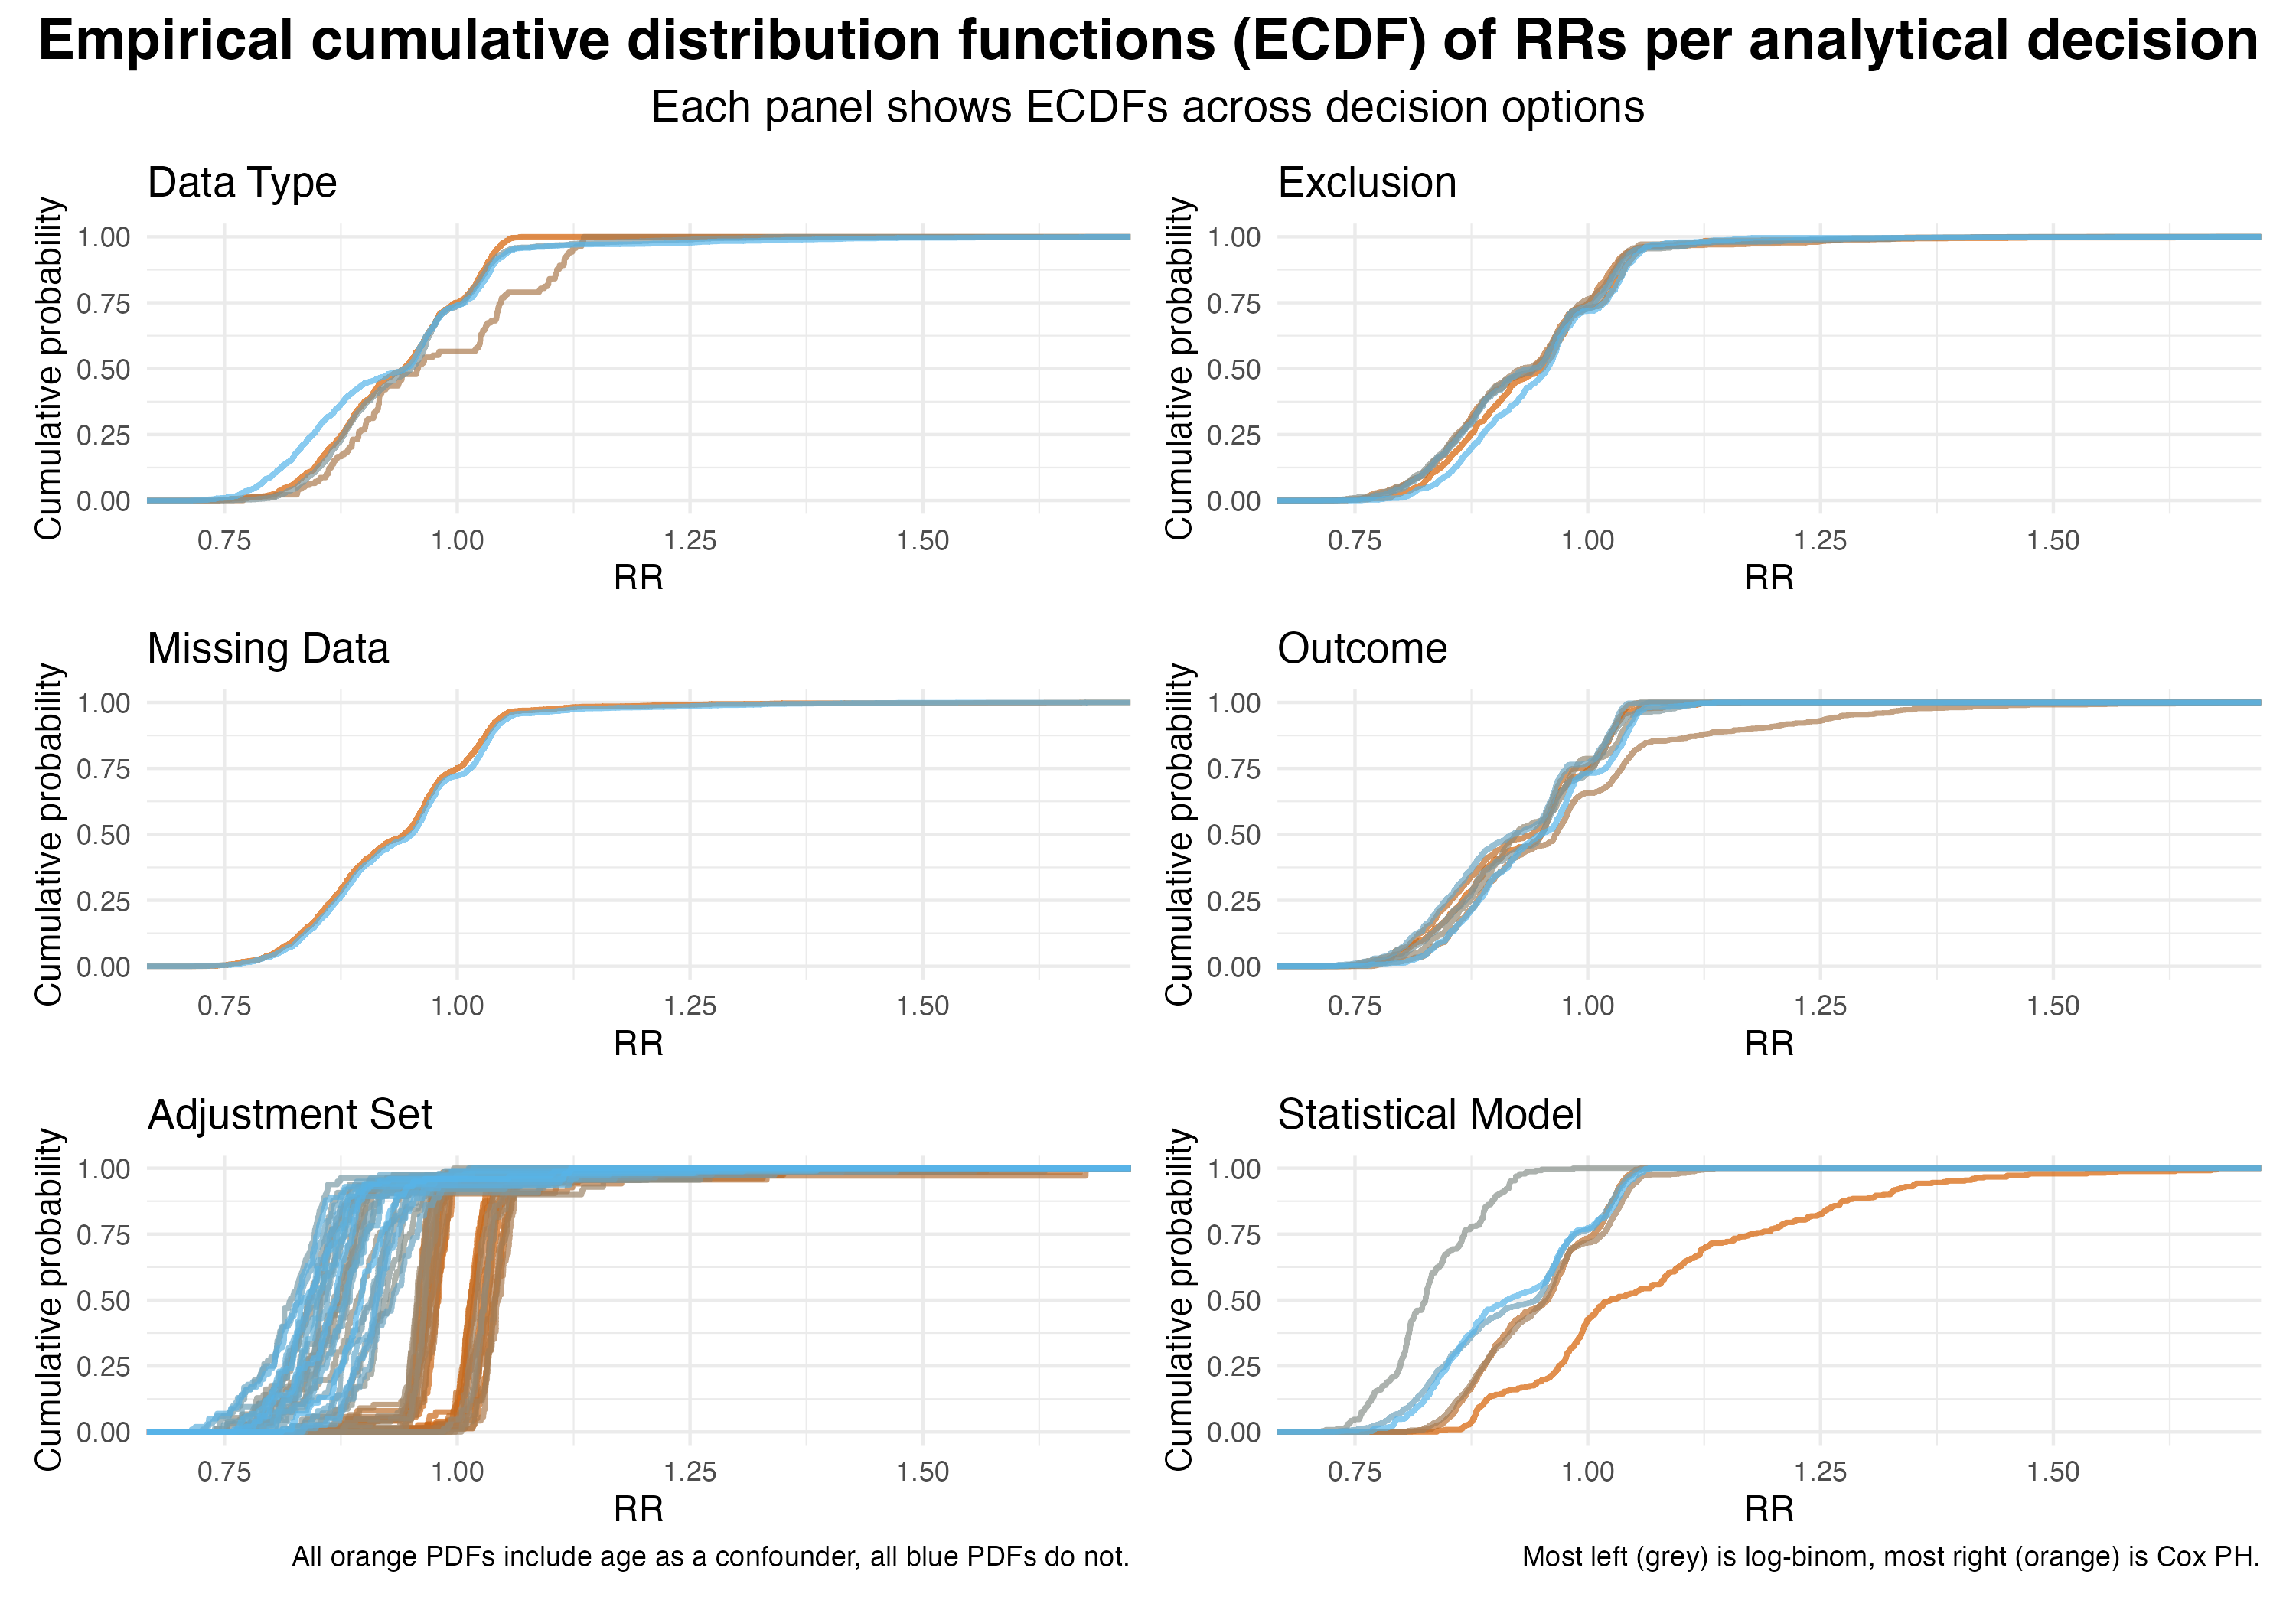
\includegraphics[width=1\linewidth,height=\textheight,keepaspectratio]{../figures/ECDF_plot.png}

\end{figure}%

\section{Empirical Cumulative Distribution Functions Per Adjustment
Variable}\label{apx-empirical-cumulative-distribution-functions-per-adjustment-variable}

\begin{figure}[H]

\caption{\label{fig-ECDF-ADJ}Empirical cumulative distribution functions
of risk ratios (RR) across inclusion/exclusion of different adjustment
variables.}

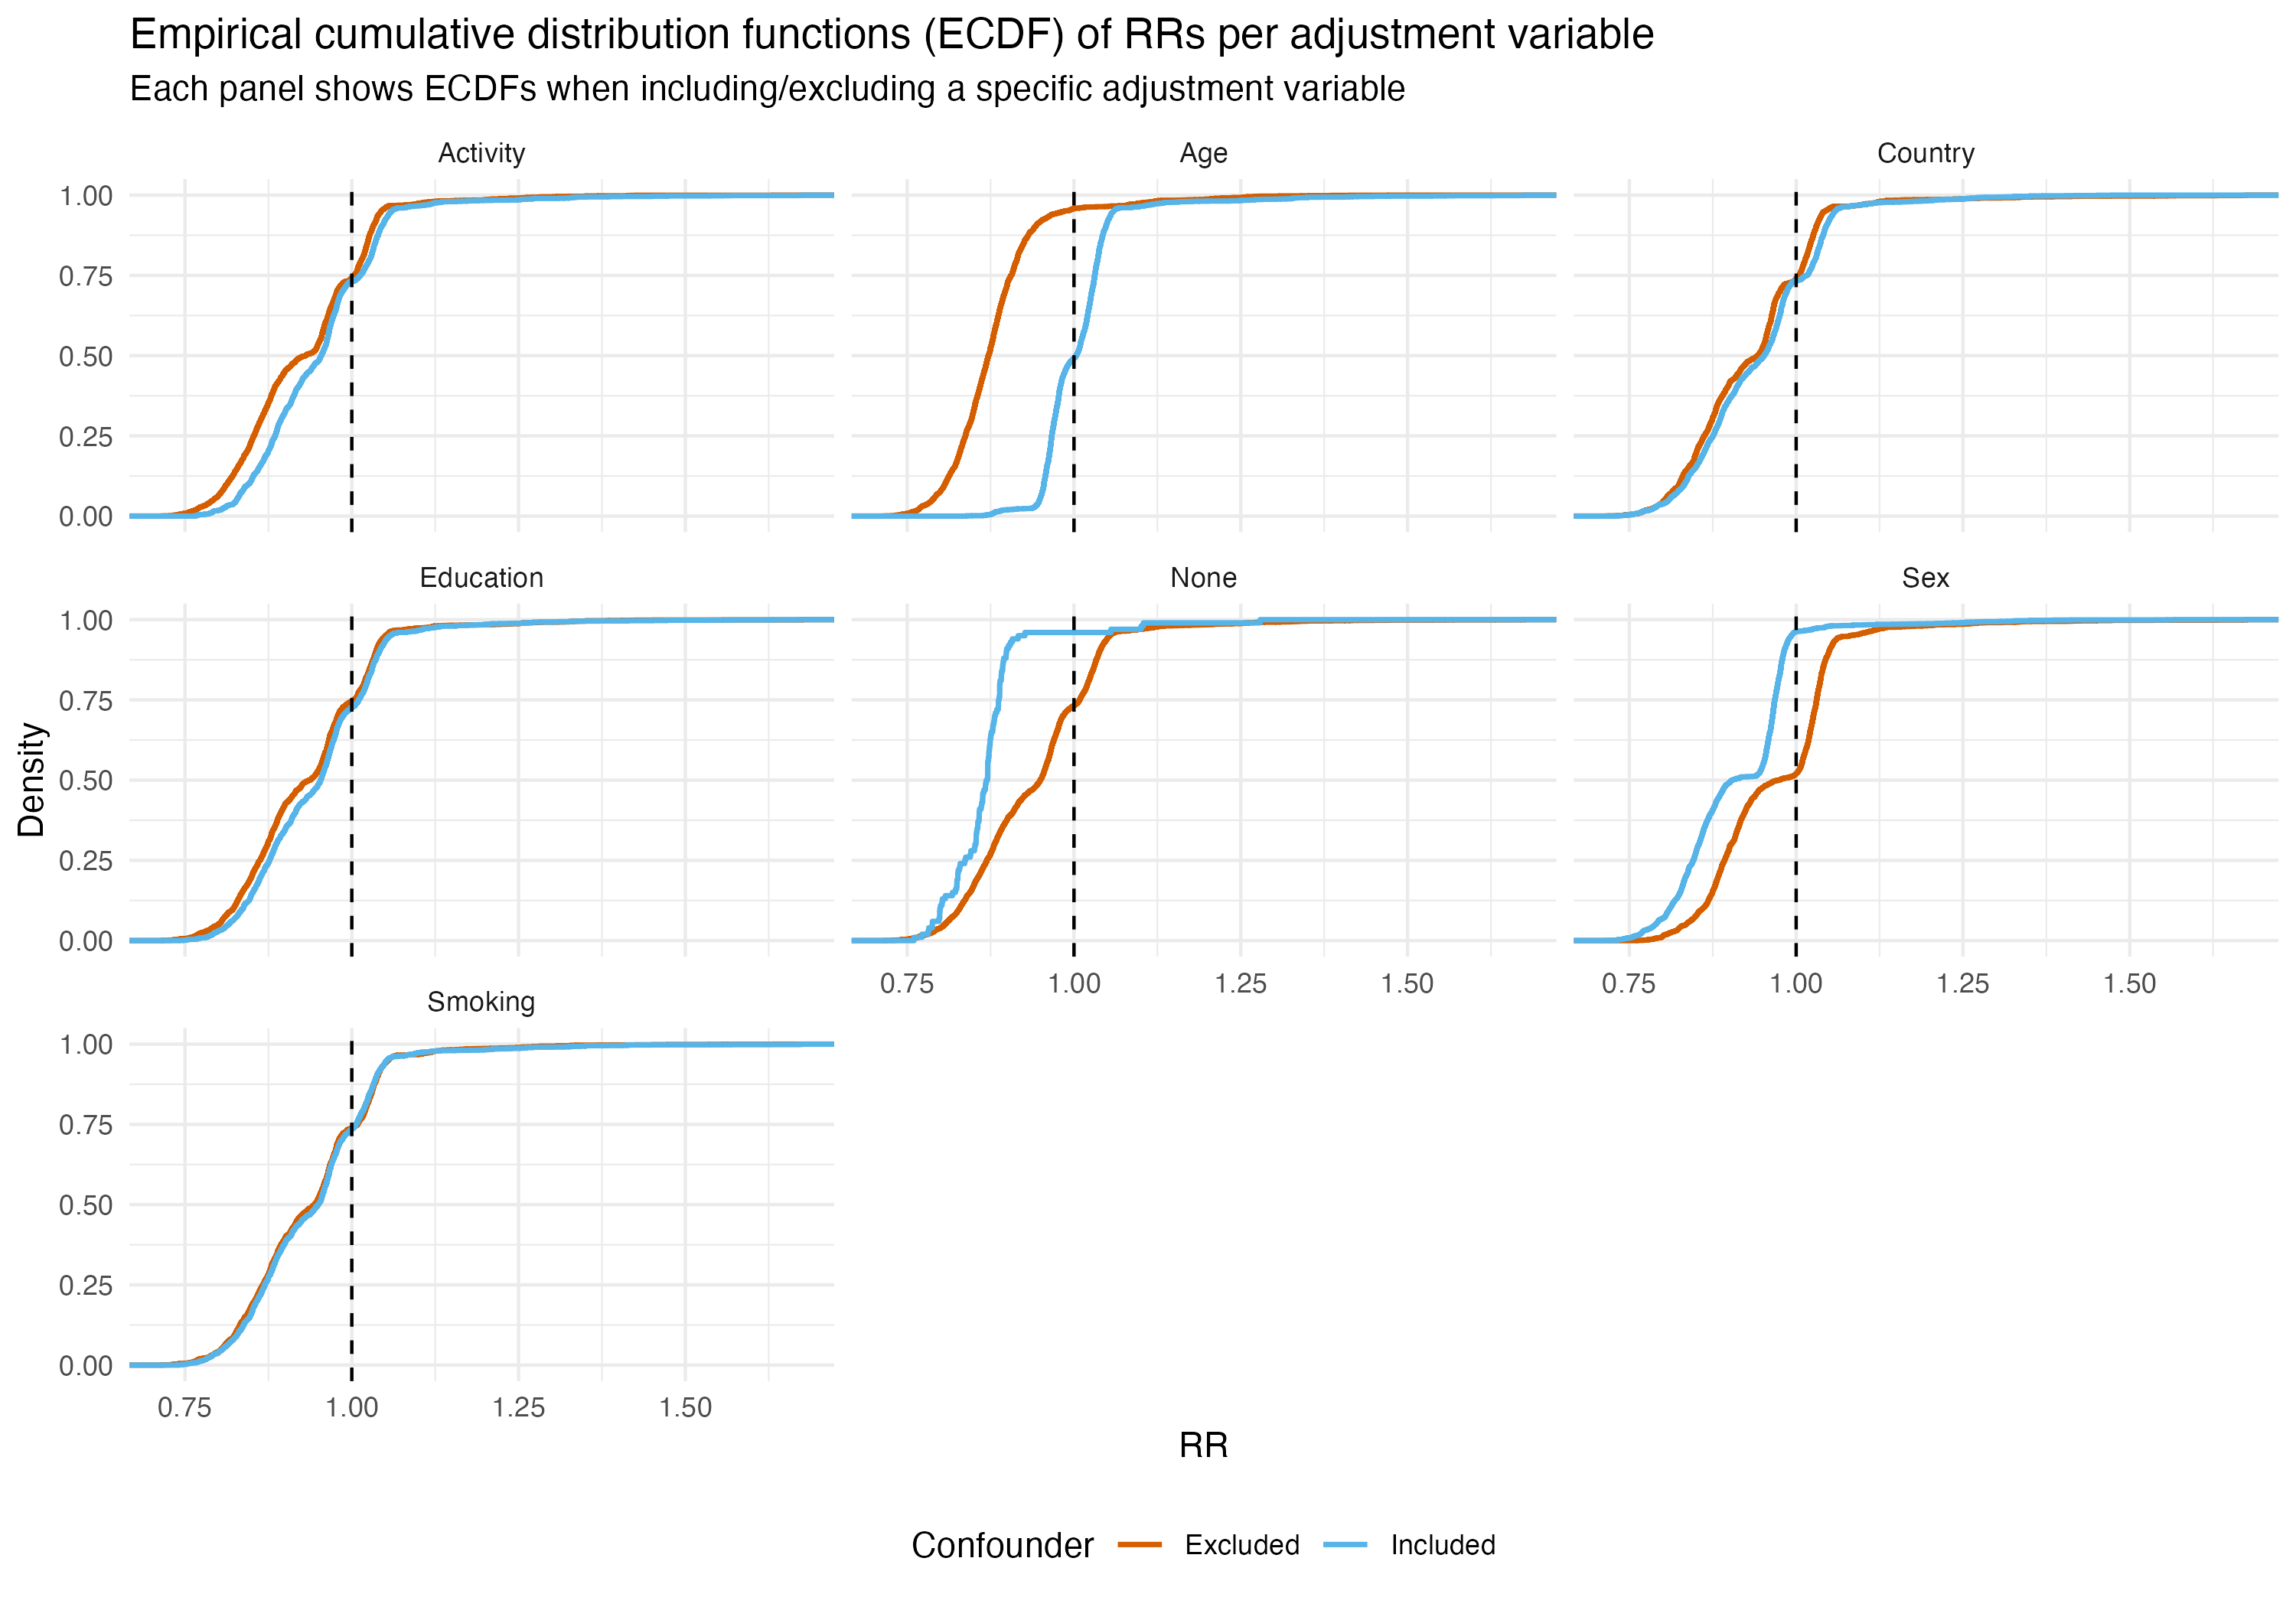
\includegraphics[width=1\linewidth,height=\textheight,keepaspectratio]{../figures/ECDF_per_confounder.png}

\end{figure}%

\section{Full Results Table}\label{apx-full-results-table}

\begingroup\fontsize{6.5}{8.5}\selectfont

\begin{longtable}[t]{>{\raggedright\arraybackslash}p{2.5cm}>{\raggedright\arraybackslash}p{5cm}>{\raggedleft\arraybackslash}p{1.2cm}>{\raggedleft\arraybackslash}p{1.2cm}>{\raggedleft\arraybackslash}p{1.5cm}>{\centering\arraybackslash}p{2cm}>{\raggedleft\arraybackslash}p{1.2cm}}

\caption{\label{tbl-RRfulltable}Number of universes including specific
decision options, non-convergence, RRs, their range and percentage of
significant RRs across decisions and their options.}

\tabularnewline

\toprule
Decision & Option & Successful Universes & Non-convergence & Mean RR & RR Range & \% Sig\\
\midrule
\endfirsthead
\multicolumn{7}{@{}l}{\textit{(continued)}}\\
\toprule
Decision & Option & Successful Universes & Non-convergence & Mean RR & RR Range & \% Sig\\
\midrule
\endhead

\endfoot
\bottomrule
\endlastfoot
Statistical Model & Log-binomial & 232 & 1102 & 0.83 & {}[0.71, 0.98] & 100\%\\
Statistical Model & Mixed effects logistic regression & 1278 & 0 & 0.92 & {}[0.73, 1.07] & 77\%\\
Statistical Model & Discrete-time mixed effects & 832 & 0 & 0.92 & {}[0.76, 1.07] & 74\%\\
Statistical Model & GEE & 1052 & 221 & 0.95 & {}[0.8, 1.06] & 85\%\\
Statistical Model & Logistic regression & 1188 & 164 & 0.95 & {}[0.8, 1.14] & 93\%\\
Statistical Model & Cox PH & 331 & 0 & 1.08 & {}[0.84, 1.68] & 24\%\\
Data Type & Cross-sectional (all waves) & 1237 & 403 & 0.93 & {}[0.74, 1.07] & 91\%\\
Data Type & Longitudinal (wave 1) & 1669 & 563 & 0.93 & {}[0.71, 1.68] & 69\%\\
Data Type & Longitudinal (no strict baseline) & 1869 & 411 & 0.95 & {}[0.75, 1.35] & 82\%\\
Data Type & Cross-sectional (wave 1) & 138 & 110 & 0.97 & {}[0.77, 1.14] & 86\%\\
Missing Data & Complete cases & 2584 & 637 & 0.94 & {}[0.72, 1.68] & 80\%\\
Missing Data & No information & 2329 & 850 & 0.94 & {}[0.71, 1.68] & 80\%\\
Exclusion Criteria & Country & 833 & 261 & 0.93 & {}[0.73, 1.54] & 76\%\\
Exclusion Criteria & Divorced/widowed & 819 & 277 & 0.93 & {}[0.73, 1.47] & 79\%\\
Exclusion Criteria & Married before 18 & 778 & 248 & 0.94 & {}[0.71, 1.45] & 82\%\\
Exclusion Criteria & None & 804 & 263 & 0.94 & {}[0.73, 1.56] & 80\%\\
Exclusion Criteria & Born after 1954 & 886 & 209 & 0.95 & {}[0.74, 1.68] & 83\%\\
Exclusion Criteria & Younger than 55 & 793 & 229 & 0.95 & {}[0.76, 1.67] & 79\%\\
Outcome & Age event + Death + Event ever + Since & 644 & 193 & 0.92 & {}[0.73, 1.06] & 84\%\\
Outcome & Death + Event ever + Since & 656 & 182 & 0.92 & {}[0.71, 1.06] & 84\%\\
Outcome & Age event + Death + Event ever & 707 & 177 & 0.93 & {}[0.75, 1.16] & 76\%\\
Outcome & Age event + Event ever + Since & 617 & 216 & 0.93 & {}[0.74, 1.07] & 86\%\\
Outcome & Death + Event ever & 761 & 187 & 0.93 & {}[0.72, 1.13] & 76\%\\
Outcome & Event ever & 695 & 266 & 0.95 & {}[0.73, 1.14] & 83\%\\
Outcome & Age event + Event ever & 833 & 266 & 0.98 & {}[0.77, 1.68] & 72\%\\
Adjustment Set & Smoke + Sex & 81 & 19 & 0.83 & {}[0.74, 1.35] & 97\%\\
Adjustment Set & Country + Sex & 100 & 0 & 0.83 & {}[0.73, 1.12] & 95\%\\
Adjustment Set & Sex & 100 & 0 & 0.83 & {}[0.71, 1.22] & 93\%\\
Adjustment Set & Smoke + Edu + Sex & 65 & 35 & 0.84 & {}[0.75, 1.01] & 93\%\\
Adjustment Set & Smoke + Country + Edu + Sex & 74 & 26 & 0.85 & {}[0.74, 1.16] & 94\%\\
Adjustment Set & Smoke + Country + Sex & 85 & 15 & 0.85 & {}[0.75, 1.03] & 90\%\\
Adjustment Set & Edu + Sex & 75 & 25 & 0.85 & {}[0.76, 1.31] & 90\%\\
Adjustment Set & Sex + Phys & 100 & 0 & 0.85 & {}[0.76, 1.39] & 94\%\\
Adjustment Set & Smoke & 86 & 14 & 0.86 & {}[0.77, 1.08] & 98\%\\
Adjustment Set & Smoke + Edu + Sex + Phys & 66 & 34 & 0.86 & {}[0.77, 1.2] & 96\%\\
Adjustment Set & Country + Edu + Sex & 73 & 27 & 0.86 & {}[0.75, 1.22] & 91\%\\
Adjustment Set & Country + Sex + Phys & 79 & 21 & 0.86 & {}[0.77, 1.01] & 97\%\\
Adjustment Set & Edu + Sex + Phys & 68 & 32 & 0.86 & {}[0.8, 1.02] & 96\%\\
Adjustment Set & Smoke + Country + Edu + Sex + Phys & 63 & 37 & 0.87 & {}[0.78, 1] & 93\%\\
Adjustment Set & Smoke + Country + Sex + Phys & 72 & 28 & 0.87 & {}[0.77, 1.21] & 92\%\\
Adjustment Set & Smoke + Sex + Phys & 84 & 16 & 0.87 & {}[0.8, 1.38] & 94\%\\
Adjustment Set & None & 100 & 0 & 0.87 & {}[0.76, 1.28] & 97\%\\
Adjustment Set & Smoke + Country & 87 & 13 & 0.88 & {}[0.78, 1.26] & 96\%\\
Adjustment Set & Country & 100 & 0 & 0.88 & {}[0.76, 1.24] & 98\%\\
Adjustment Set & Country + Edu + Sex + Phys & 73 & 27 & 0.89 & {}[0.79, 1.25] & 91\%\\
Adjustment Set & Edu & 78 & 22 & 0.89 & {}[0.79, 1.13] & 99\%\\
Adjustment Set & Smoke + Country + Edu & 66 & 34 & 0.90 & {}[0.79, 1.21] & 93\%\\
Adjustment Set & Smoke + Edu & 67 & 33 & 0.90 & {}[0.79, 1.41] & 95\%\\
Adjustment Set & Phys & 100 & 0 & 0.90 & {}[0.81, 1.12] & 100\%\\
Adjustment Set & Country + Edu & 75 & 25 & 0.91 & {}[0.81, 1.21] & 93\%\\
Adjustment Set & Smoke + Country + Phys & 84 & 16 & 0.92 & {}[0.82, 1.1] & 94\%\\
Adjustment Set & Smoke + Phys & 87 & 13 & 0.92 & {}[0.81, 1.25] & 93\%\\
Adjustment Set & Country + Phys & 100 & 0 & 0.92 & {}[0.82, 1.31] & 96\%\\
Adjustment Set & Edu + Phys & 79 & 21 & 0.93 & {}[0.83, 1.24] & 98\%\\
Adjustment Set & Smoke + Country + Edu + Phys & 69 & 31 & 0.94 & {}[0.83, 1.27] & 95\%\\
Adjustment Set & Smoke + Edu + Phys & 75 & 25 & 0.94 & {}[0.84, 1.47] & 95\%\\
Adjustment Set & Country + Edu + Phys & 72 & 28 & 0.94 & {}[0.83, 1.27] & 92\%\\
Adjustment Set & Age + Smoke + Sex & 74 & 26 & 0.96 & {}[0.87, 1.24] & 82\%\\
Adjustment Set & Age + Country + Edu + Sex & 69 & 31 & 0.96 & {}[0.87, 1.02] & 63\%\\
Adjustment Set & Age + Edu + Sex & 60 & 40 & 0.96 & {}[0.88, 1.09] & 80\%\\
Adjustment Set & Age + Sex & 82 & 18 & 0.96 & {}[0.88, 1.03] & 88\%\\
Adjustment Set & Age + Smoke + Country + Edu + Sex & 62 & 38 & 0.97 & {}[0.84, 1.3] & 69\%\\
Adjustment Set & Age + Smoke + Edu + Sex & 68 & 32 & 0.97 & {}[0.89, 1.41] & 79\%\\
Adjustment Set & Age + Smoke + Sex + Phys & 79 & 21 & 0.97 & {}[0.9, 1.33] & 77\%\\
Adjustment Set & Age + Country + Sex & 77 & 23 & 0.97 & {}[0.87, 1.28] & 68\%\\
Adjustment Set & Age + Sex + Phys & 79 & 21 & 0.97 & {}[0.88, 1.56] & 78\%\\
Adjustment Set & Age + Smoke + Country + Edu + Sex + Phys & 61 & 39 & 0.98 & {}[0.88, 1.26] & 54\%\\
Adjustment Set & Age + Smoke + Country + Sex & 75 & 25 & 0.98 & {}[0.84, 1.35] & 65\%\\
Adjustment Set & Age + Smoke + Edu + Sex + Phys & 62 & 38 & 0.98 & {}[0.88, 1.57] & 80\%\\
Adjustment Set & Age + Country + Edu + Sex + Phys & 80 & 20 & 0.98 & {}[0.87, 1.33] & 57\%\\
Adjustment Set & Age + Country + Sex + Phys & 86 & 14 & 0.98 & {}[0.85, 1.33] & 57\%\\
Adjustment Set & Age + Edu + Sex + Phys & 65 & 35 & 0.98 & {}[0.88, 1.33] & 76\%\\
Adjustment Set & Age + Smoke + Country + Sex + Phys & 72 & 28 & 0.99 & {}[0.87, 1.32] & 43\%\\
Adjustment Set & Age + Smoke & 75 & 25 & 1.01 & {}[0.92, 1.04] & 37\%\\
Adjustment Set & Age & 87 & 13 & 1.02 & {}[0.98, 1.42] & 33\%\\
Adjustment Set & Age + Smoke + Edu & 80 & 20 & 1.02 & {}[0.96, 1.13] & 27\%\\
Adjustment Set & Age + Smoke + Edu + Phys & 61 & 39 & 1.03 & {}[0.94, 1.67] & 51\%\\
Adjustment Set & Age + Smoke + Country & 73 & 27 & 1.04 & {}[0.95, 1.42] & 44\%\\
Adjustment Set & Age + Smoke + Country + Edu & 67 & 33 & 1.04 & {}[0.96, 1.2] & 60\%\\
Adjustment Set & Age + Smoke + Country + Edu + Phys & 66 & 34 & 1.04 & {}[0.94, 1.45] & 77\%\\
Adjustment Set & Age + Country & 87 & 13 & 1.04 & {}[0.98, 1.28] & 74\%\\
Adjustment Set & Age + Edu & 71 & 29 & 1.04 & {}[0.99, 1.63] & 48\%\\
Adjustment Set & Age + Phys & 85 & 15 & 1.04 & {}[0.98, 1.34] & 60\%\\
Adjustment Set & Age + Smoke + Country + Phys & 78 & 22 & 1.05 & {}[0.98, 1.4] & 82\%\\
Adjustment Set & Age + Smoke + Phys & 68 & 32 & 1.05 & {}[0.97, 1.68] & 58\%\\
Adjustment Set & Age + Country + Edu & 63 & 37 & 1.05 & {}[0.98, 1.37] & 75\%\\
Adjustment Set & Age + Country + Edu + Phys & 71 & 29 & 1.05 & {}[1, 1.47] & 78\%\\
Adjustment Set & Age + Country + Phys & 77 & 23 & 1.05 & {}[0.99, 1.45] & 70\%\\
Adjustment Set & Age + Edu + Phys & 70 & 30 & 1.05 & {}[1, 1.54] & 59\%\\*

\end{longtable}

\endgroup{}






\end{document}
